%\nocite{b28b8d8f}
%\nocite{4dd1b85f}
%\nocite{a565d200}
%\nocite{c82f5e22}
%\nocite{4dc38f27}
%\nocite{d09756a3}
%\nocite{6d9ad807}
%\nocite{00000011}
%TODO
%  formalize internal nerve
Simplicial sets model homotopy types as well as topological spaces do. This can be made formal using an equivalence on a $(\infty,1)$-topos level or more commonly (but essentially equivalent) a \textit{Quillen equivalence} on the \textit{model category}\footnote{we will briefly allude to them in the next section \ref{sec:fibration}} level. However, we will not really discuss this in this generality in this section. This was just the attention-getter. Yet, it should become clear on a more intuitive level that it works. For we will explain how one can build a CW complex from a simplicial set which will be a certain presheaf consisting of {\glqq}triangles of any dimension{\grqq}. One calls this geometric realization of the simplicial set. Before we do this we provide motivation for simplicial sets - combinatorial and geometrical - and compare a bit to the traditional notion of the quite rigid \textit{simplicial complexes}. We then geometrically motivate how we can utilize the machinery developed in subsubsection \ref{sec:coyoneda2} to geometrically realize with the Kan extenstions of the Yoneda functor. The same machinery applies for truncation of higher homotopy information as we will see when it comes to the nerve functor. This naturally leads to thoughts about the classification of principal bundles in $\mathbf{Top}$ by certain homotopy classes and then \v{C}ech cohomology which then in turn classify these homotopy classes. We conclude the section with a sequel of the generalized spaces example.
\\\\
To start off with, if you know some algebraic topology you might know simplicial complexes which are special cases of simplicial sets in that we allow for degenerate simplices in all dimensions in simplicial sets. This means that e.g. a point or a line can be considered a triangle. This is what makes simplicial sets way more flexible (just like a CW complex) than the rigid simplicial complexes. However, if you do not know simplicial complexes this does not help you much and we try to start from scratch. First we have to settle the question what a simplex of some dimension means. Well an $N$-simplex for $N \in \mathbb{N}$ shall be an $N$-dimensional version of a triangle. Geometrically, for $N \in \mathbb{N}$ the set
\begin{align*}
  \blacktriangle^{[N]}
  &:=
  \left\lbrace
      (x_{1},x_{2},\ldots,x_{N+1})
      \in
      \mathbb{R}^{N+1}
    \,
    \vert
    \,
      x_{i}
      \in
      [0,1]
      \,
      \land
      \,
      \sum_{i=1}^{N+1}
      x_{i}
      =
      1
  \right\rbrace
\end{align*}
topologized by the $\mathbb{R}^{N+1}$ subspace topology is called \textbf{$N$(-dimensional topological standard) simplex} which is just expressed by $N$-simplex. Let us illustrate the case $N = 0,1,2$ by
\[
\begin{tikzpicture}[scale=0.75]
  \fill[fill=green]
    (2,0) node[below] {$1$}
    circle
    (2pt);
  \draw[->]
    (0,0)
    --
    (4,0) node[right] {$x_{1}$};
\end{tikzpicture}
\]
\[
\begin{tikzpicture}[scale=0.75]
  \fill
    (2,0) node[below] {$1$}
    --
    (0,2) node[left] {$1$};
  \draw[green]
    (2,0)
    --
    (0,2);
  \draw[->]
    (0,0)
    --
    (4,0) node[right] {$x_{1}$};
  \draw[->]
    (0,0)
    --
    (0,4) node[above] {$x_{2}$};
\end{tikzpicture}
\]
\[
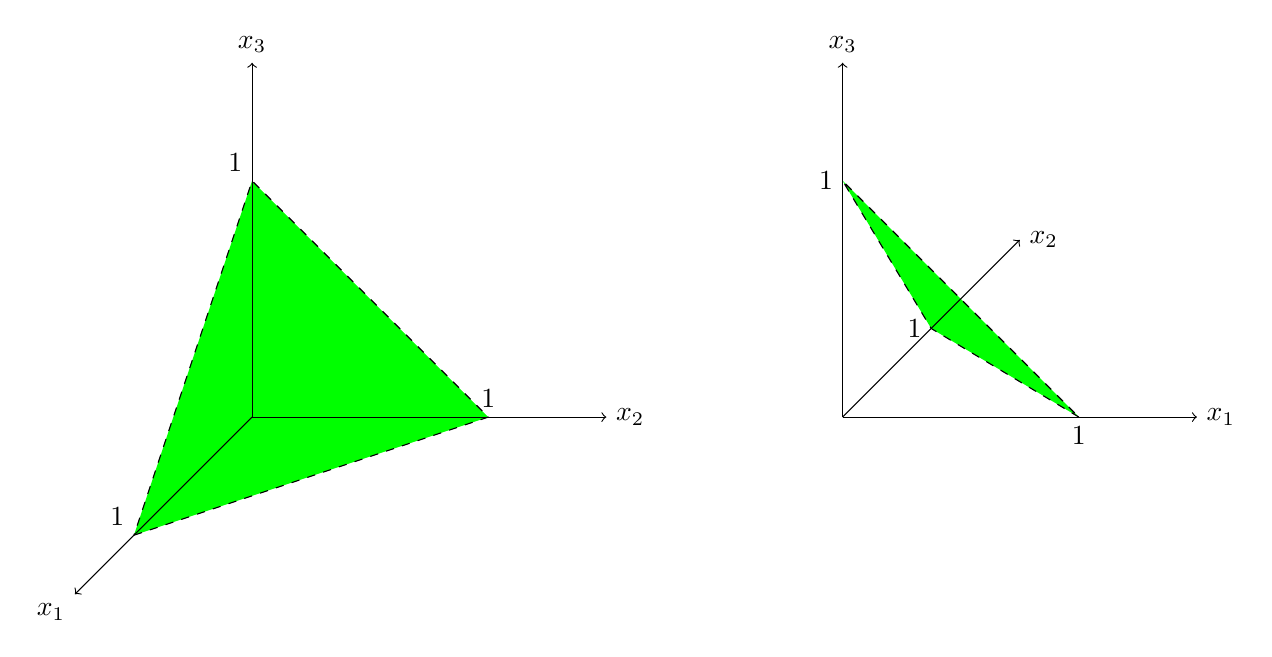
\begin{tikzpicture}[scale=0.75]
  \filldraw[dashed,fill=green]
    (-7,-2) node[above left] {$1$}
    --
    (-1,0) node[above] {$1$}
    --
    (-5,4) node[above left] {$1$}
    --
    cycle;
  \draw[->]
    (-5,0)
    --
    (-8,-3) node[below left] {$x_{1}$};
  \draw[->]
    (-5,0)
    --
    (1,0) node[right] {$x_{2}$};
  \draw[->]
    (-5,0)
    --
    (-5,6) node[above] {$x_{3}$};
  \filldraw[dashed,fill=green]
    (9,0) node[below] {$1$}
    --
    (6.5,1.5) node[left] {$1$}
    --
    (5,4) node[left] {$1$}
    --
    cycle;
  \draw[->]
    (5,0)
    --
    (11,0) node[right] {$x_{1}$};
  \draw[->]
    (5,0)
    --
    (8,3) node[right] {$x_{2}$};
  \draw[->]
    (5,0)
    --
    (5,6) node[above] {$x_{3}$};
\end{tikzpicture}
\]
$\blacktriangle^{[2]}$ is the triangle bounded by the dashed lines. Unfortunately, we cannot draw higher dimensions this way but $N = 3$ would be pyramid-shaped which can at least be illustrated as
\[
\begin{tikzpicture}[scale=0.75]
  \draw
    (-2,-2) 
    --
    (4,0)
    --
    (0,4)
    --
    cycle;
  \draw
    (0,0)
    --
    (-2,-2);
  \draw
    (0,0)
    --
    (4,0);
  \draw
    (0,0)
    --
    (0,4);
\end{tikzpicture}
\]
Now how can we capture this geometric information combinatorially? Actually, it suffices to know the dimension of the standard simplex we want to draw. So combinatorially we can consider the $N$-dimensional standard simplex as the set
\begin{align*}
  [N]
  &:=
  \lbrace
      n
      \in
      \mathbb{N}^{\times}
    \,
    \vert
    \,
      n
      \leq
      N
      +
      1
  \rbrace
\end{align*}
for all $N \in \mathbb{N}$ where we can consider the elements of $[N]$ as the corners of the $N$-simplex. In this way we have a natural order of the corners which is reflected as induced well-order on $[N]$ by the well-order of the natural number. Let us denote this
\begin{align*}
  [N]
  \doteq
  ([N],\leq)
  &\doteq
  ([N],\leq_{[N]})
\end{align*}
where $\leq_{[N]}$ is the restriction of the standard well-order $\leq_{\mathbb{N}}$ on the natural numbers. But $\blacktriangle^{[N]}$ contains even more information. Namely all the standard simplices of dimension lower than $N$ which can be embedded in the $N$-dimensional topological simplex in an order-preserving way. That is, we can restrict the $N$-dimensional topological simplex to get those of lower dimension. For example we have three possibilities of embedding the $1$-dimensional topological simplex into the $2$-dimensional topological simplex in an order-preserving way indicated by the following picture
\[
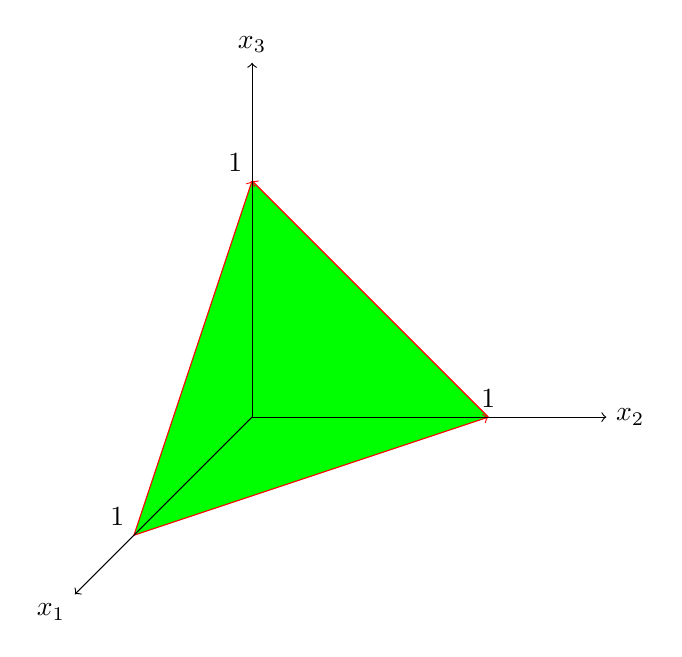
\begin{tikzpicture}[scale=0.75]
  \fill[fill=green]
    (-2,-2) node[above left] {$1$}
    --
    (4,0) node[above] {$1$}
    --
    (0,4) node[above left] {$1$}
    --
    cycle;
  \draw[->,red]
    (-2,-2)
    --
    (4,0);
  \draw[->,red]
    (-2,-2)
    --
    (0,4);
  \draw[->,red]
    (4,0)
    --
    (0,4);
  \draw[->]
    (0,0)
    --
    (-3,-3) node[below left] {$x_{1}$};
  \draw[->]
    (0,0)
    --
    (6,0) node[right] {$x_{2}$};
  \draw[->]
    (0,0)
    --
    (0,6) node[above] {$x_{3}$};
\end{tikzpicture}
\]
where the arrows symbolize the order of the embedded $1$-dimensional topological simplex. Combinatorially, we get for $i \in [N]$ functions
\begin{align*}
  \delta_{N,i}
  \colon
  [N-1]
  &\rightarrow
  [N]
  \\
  n
  &\mapsto
  \begin{cases}
    n
    &
    \text{for }
    n
    <
    i
    \\
    n
    +
    1
    &
    \text{for }
    n
    \geq
    i
  \end{cases}
\end{align*}
$\delta_{N,i}$ are precisely the strictly\footnote{with $<$ instead of $\leq$ in the order-preserving definition} order-preserving functions from $[N-1]$ to $[N]$. Even better: for all $N > 0$ the strictly order-preserving functions from $[N-k]$ to $[N]$ with $1 \leq k \leq N$ always decompose (not uniquely in general) as
\begin{align*}
  \delta_{N,i_{N}}
  \circ
  \cdots
  \circ
  \delta_{N-k+1,i_{N-k+1}}
\end{align*}
for some combination $(i_{N-k+1},\ldots,i_{N})$. But this shall not concern us here much. More important is the observation that restricting the object set of the category of well-ordered sets $\mathbf{WO}$ (see subsection \ref{sec:cat}) to only the well-ordered sets of the sort $([N],\leq)$ for some $N$ yields a full subcategory $\mathbf{\Delta}$. We call $\mathbf{\Delta}$ the \textbf{simplex category}.\footnote{note that $([N],\leq)$ corresponds itself to a category - the poset-category (again see subsection \ref{sec:cat}) - but this will only be important in construction \ref{cst:nerve} below} You might object that according to the above we should restrict $\mathbf{\Delta}$ to the subcategory $\mathbf{\Delta}_{\neq}$ with only \underline{strictly} order-preseving functions. For the record: let us call $\mathbf{\Delta}_{\neq}$ the \textbf{strict simplex category}. One can do that and in some cases it might be reasonable but usually it is an artifical restriction yielding a too rigid construction to be feasible in many applications. This is because if we take any order-preserving function into account then we in particular have order-preserving functions
\begin{align*}
  \sigma_{N,i}
  \colon
  [N + 1]
  &\rightarrow
  [N]
  \\
  n
  &\mapsto
  \begin{cases}
    n
    &
    \text{for }
    n
    \leq
    i
    \\
    n
    -
    1
    &
    \text{for }
    n
    >
    i
  \end{cases}
\end{align*}
for $i \in [N]$. And if the $\delta_{N,i}$ tell how we can restrict to lower dimension then the $\sigma_{N,i}$ must tell how we can consider $N$-dimensions as {\glqq}degenerated{\grqq} $N+1$-dimensions. This is to say that e.g. a point or a line are a degenerated triangle. This is the point where the flexibility of the soon defined simplicial sets originates from. Furthermore note that one can show that a morphism in $\mathbf{\Delta}$ decomposes as a combination of all $\delta_{N_{1},i}$ and all $\sigma_{N_{2},i}$ for $N_{1},N_{2} \in \mathbb{N}$ in an analogous manner as above where all non-identity morphisms in $\mathbf{\Delta}_{\neq}$ decomposed as a combination of $\delta_{N,i}$. But also this fact shall not concern us much here. After all we can define functors
\begin{align*}
  \vert
    \cdot
  \vert^{\textrm{stand}}
  \colon
  \mathbf{\Delta}
  &\rightarrow
  \mathbf{Top}
  \\
  [N]
  &\mapsto
  \blacktriangle^{[N]}
  \\
  \left(
    f
    \colon
    [N_{1}]
    \rightarrow
    [N_{2}]
  \right)
  &\mapsto
  \left(
    \sum_{i=1}^{N_{1}+1}
    x_{i}e_{i}
    \mapsto
    \sum_{i=1}^{N_{1}+1}
    x_{i}e_{f(i)}
  \right)
  \\\\
  \vert
    \cdot
  \vert_{\neq}^{\textrm{stand}}
  \colon
  \mathbf{\Delta}_{\neq}
  &\rightarrow
  \mathbf{Top}
  \\
  [N]
  &\mapsto
  \blacktriangle^{[N]}
  \\
  \left(
    f
    \colon
    [N_{1}]
    \rightarrow
    [N_{2}]
  \right)
  &\mapsto
  \left(
    \sum_{i=1}^{N_{1}+1}
    x_{i}e_{i}
    \mapsto
    \sum_{i=1}^{N_{1}+1}
    x_{i}e_{f(i)}
  \right)
\end{align*}
where $e_{i}$ denotes the $i$-th canonical basis vector of $\mathbb{R}^{n}$. We call $\vert \cdot \vert^{\textrm{stand}}$ the \textbf{geometric realization (of the standard simplices)} while $\vert \cdot \vert_{\neq}^{\textrm{stand}}$ is called the \textbf{geometric realization (of the strict standard simplices)}.
\\\\
Now what is the purpose of simplices? Well, in classical homotopy theory one usually tries to divide a space into simpler pieces which one knows very well from a homotopy perspective in a manner preserving the homotopy structure. The usual way to do this are CW complexes which model a space by balls of any dimension (this always works up to coherent homotopy). But in classical homotopy theory with topological spaces there is no combinatorial counterpart.\footnote{in UFP-HoTT the distinction becomes a bit more blurry (which is good in this case)} Therefore one used to take so-called simplicial complexes in the early days of algebraic topology. Loosely speaking, one divides a space into simplices of any dimension that allows for a combinatorial treatment. However, one needs many simplices to divide up comparably simple spaces such as a torus, for example: note that a (topological) torus is often defined as the space $[0,1] \times [0,1]$ modulo the equivalence relation generated by
\begin{align*}
  (0,t)
  &\sim
  (1,t)
  \\
  (t,0)
  &\sim
  (t,1)
\end{align*}
This is illustrated by
\[
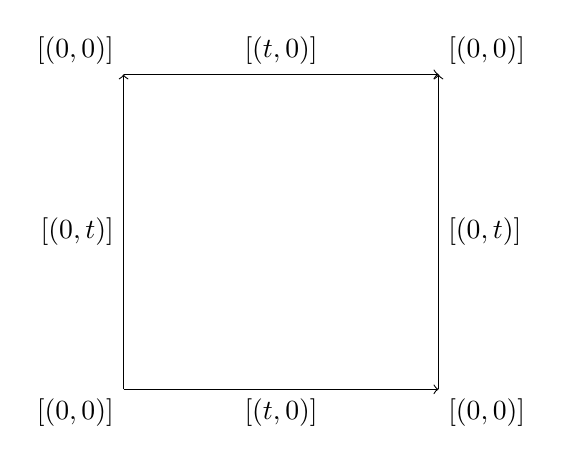
\begin{tikzpicture}[scale=4]
  \draw[->]
    (0,0) node[below left] {$[(0,0)]$}
    -- node[below] {$[(t,0)]$}
    (1,0) node[below right] {$[(0,0)]$};
  \draw[->]
    (0,1) node[above left] {$[(0,0)]$}
    -- node[above] {$[(t,0)]$}
    (1,1) node[above right] {$[(0,0)]$};
  \draw[->]
    (0,0)
    -- node[left] {$[(0,t)]$}
    (0,1) ;
  \draw[->]
    (1,0)
    -- node[right] {$[(0,t)]$}
    (1,1);
\end{tikzpicture}
\]
and we would like to divide the torus up in
\begin{enumerate}
\item[$\bullet$]
$2$ triangles $\triangle_{1}$ and $\triangle_{2}$
\item[$\bullet$]
$3$ lines $\upharpoonleft$, $\rightharpoonup$ and $\nearrow$
\item[$\bullet$]
$1$ corner $\centerdot$
\end{enumerate}
as illustrated by
\[
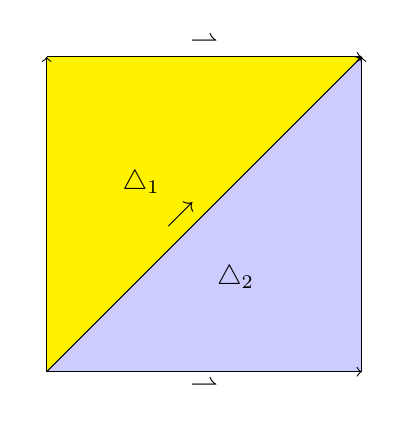
\begin{tikzpicture}[scale=4]
  \fill[yellow]
    (0,0)
    --
    (0,1)
    --
    (1,1)
    --
    cycle;
  \fill[blue!20]
    (0,0)
    --
    (1,0)
    --
    (1,1)
    --
    cycle;
  \draw
    (0.3,0.6) node {$\triangle_{1}$};
  \draw
    (0.6,0.3) node {$\triangle_{2}$};
  \draw[->]
    (0,0) node[below left] {$\centerdot$}
    -- node[below] {$\rightharpoonup$}
    (1,0) node[below right] {$\centerdot$};
  \draw[->]
    (0,1) node[above left] {$\centerdot$}
    -- node[above] {$\rightharpoonup$}
    (1,1) node[above right] {$\centerdot$};
  \draw[->]
    (0,0)
    -- node[left] {$\nearrow$}
    (1,1);
  \draw[->]
    (0,0)
    -- node[left] {$\upharpoonleft$}
    (0,1);
  \draw[->]
    (1,0)
    -- node[right] {$\upharpoonleft$}
    (1,1);
\end{tikzpicture}
\]
We do not want to expilcitly say here what a simplicial complex is but this is not a simplicial complex since $\triangle_{1}$ has the same faces as $\triangle_{2}$ and for a simplicial complex structure on the torus one would at least need $14$ triangles. What we rather have here are three sets
\begin{align*}
  &
  \lbrace
    \triangle_{1},
    \triangle_{2}
  \rbrace
  \\
  &
  \lbrace
    \upharpoonleft,
    \rightharpoonup,
    \nearrow
  \rbrace
  \\
  &
  \lbrace
    \centerdot
  \rbrace
\end{align*}
and
\begin{align*}
  \rightharpoonup
  &\text{ is the first face of }
  \triangle_{1}
  \\
  \nearrow
  &\text{ is the second face of }
  \triangle_{1}
  \\
  \upharpoonleft
  &\text{ is the third face of }
  \triangle_{1}
  \\
  \upharpoonleft
  &\text{ is the first face of }
  \triangle_{2}
  \\
  \nearrow
  &\text{ is the second face of }
  \triangle_{2}
  \\
  \rightharpoonup
  &\text{ is the third face of }
  \triangle_{2}
\end{align*}
Hence we can try to define a functor $\odot \colon \mathbf{\Delta}_{\neq}^{\mathrm{op}} \rightarrow \mathbf{Set}$ with
\begin{align*}
  \odot([0])
  &:=
  \lbrace
    \centerdot
  \rbrace
  \\
  \odot([1])
  &:=
  \lbrace
    \upharpoonleft,
    \rightharpoonup,
    \nearrow
  \rbrace
  \\
  \odot([2])
  &:=
  \lbrace
    \triangle_{1},
    \triangle_{2}
  \rbrace
  \\
  \odot(\delta_{2,1})
  &:=
  \lbrace
    (\triangle_{1},\rightharpoonup),
    (\triangle_{2},\upharpoonleft)
  \rbrace
  \\
  \odot(\delta_{2,2})
  &:=
  \lbrace
    (\triangle_{1},\nearrow),
    (\triangle_{2},\nearrow)
  \rbrace
  \\
  \odot(\delta_{2,3})
  &:=
  \lbrace
    (\triangle_{1},\upharpoonleft),
    (\triangle_{2},\rightharpoonup)
  \rbrace
  \\
  \odot(\delta_{1,i})
  &:=
  \lbrace
    (\rightharpoonup,\centerdot),
    (\nearrow,\centerdot),
    (\upharpoonleft,\centerdot)
  \rbrace
\end{align*}
and the obvious on the identity arrows of $\mathbf{\Delta}_{\neq}^{\mathrm{op}}$. Further we require $\odot$ to be on the composition of the various fitting $\delta_{N,i}$ such that $\odot$ respects composition and $F([N]) = \emptyset$ for $N > 2$. Then $\odot$ is apparently a functor by construction and captures the combinatorial data we imposed on the torus.
\\\\
This torus example suggests some terminology: a functor $F \colon \mathbf{\Delta}_{\neq}^{\mathrm{op}} \rightarrow \mathbf{Set}$ is called \textbf{strict simplicial set}. And we immediately generalize (as is proper for a real category theorist) to: a functor $F \colon \mathbf{\Delta}^{\mathrm{op}} \rightarrow \mathbf{Set}$ is called \textbf{simplicial set}. Note that the {\glqq}strict{\grqq} terminology is presumably not very common since we made it up. More common is semi-simplicial set or delta sets for strict simplicial sets. Altogether the terminology is historically a bit confusing and further discussed in \cite{8b5861fc} and \cite{4dd1b85f}. Both sources provide alternative intuition on the subject of strict simplicial sets and semi-simplicial sets we do not mention here. Other worthwhile sources are \cite{d09756a3} and a little more advanced \cite{b28b8d8f}. Anyways, both simplicial sets and its strict special case give rise to catgeories as functor categories
\begin{align*}
  \mathbf{sSet}_{\neq}
  &:=
  \mathbf{Set}^{\mathbf{\Delta}_{\neq}^{\mathrm{op}}}
  \\
  \mathbf{sSet}
  &:=
  \mathbf{Set}^{\mathbf{\Delta}^{\mathrm{op}}}
\end{align*}
where we call
\begin{enumerate}
\item[(1)]
$\mathbf{sSet}_{\neq}$ the \textbf{category of strict simplicial sets}
\item[(2)]
$\mathbf{sSet}$ the \textbf{category of simplicial sets}
\end{enumerate}
But this suggests what a strict simplicial map and a simplicial map shall be: natural transformations in the according category.
\begin{enumerate}
\item[(1)]
$\mathsf{S} \in \mathrm{Mor}_{\mathbf{sSet}_{\neq}}$ is called \textbf{strict simplicial map (from $\mathrm{dom}(\mathsf{S})$ to $\mathrm{cod}(\mathsf{S})$)}. For $\mathsf{S}$ being natural means that we have a family of functions
\begin{align*}
  \mathsf{S}([N])
  \colon
  \mathrm{dom}(\mathsf{S})([N])
  &\rightarrow
  \mathrm{cod}(\mathsf{S})([N])
\end{align*}
indexed by $N$. And since $\mathrm{dom}(\mathsf{S})([N])$ and $\mathrm{cod}(\mathsf{S})([N])$ are thought of as sets of $N$-simplices a strict simplicial map can be thought of as mapping simplices of a certain dimension to simplices of the same dimension. This is the same as it is for simplicial complexes. And this is where the rigid behaviour of simplicial complexes and hence strict simplicial sets comes from.
\item[(2)]
$\mathsf{S} \in \mathrm{Mor}_{\mathbf{sSet}}$ is called \textbf{simplicial map (from $\mathrm{dom}(\mathsf{S})$ to $\mathrm{cod}(\mathsf{S})$)}. For $\mathsf{S}$ being natural means that we have a family of functions
\begin{align*}
  \mathsf{S}([N])
  \colon
  \mathrm{dom}(\mathsf{S})([N])
  &\rightarrow
  \mathrm{cod}(\mathsf{S})([N])
\end{align*}
indexed by $N$. But $\mathrm{dom}(\mathsf{S})([N])$ and $\mathrm{cod}(\mathsf{S})([N])$ can now also contain degenerate $N$-simplices, that is, simplices of lower dimension than $N$ unlike in the strict case. This is to say that a simplicial map can be thought of as mapping $N$-simplices to simplices of equal or lower dimension than $N$. This is comparable to the situation of cellular maps for CW complexes which also map to lower or equal dimension. This is where the flexibility of CW complexes and hence simplicial sets comes from.\footnote{if you have worked through proofs of space approximation by simplicial complexes and CW complexes you might have recognized the convenience of CW complexes (see \cite{8b5861fc} for some possible proofs)}
\end{enumerate}
The next point is that strict simplicial sets and simplicial sets are some presheaeves on $\mathbf{\Delta}_{\neq}$ and $\mathbf{\Delta}$, respectively. According to our interpretation of presheaves in section \ref{sec:uni} we can consider them a generalized form of strict simplices and simplices, respectively, since we consider the objects of $\mathbf{\Delta}_{\neq}$ and $\mathbf{\Delta}$, respectively, as standard $N$-simplices. The standard simplices themselves can then be considered as strict simplicial sets and simplicial sets, respectively, by embedding them into presheaves by the Yoneda functor. Hence
\begin{enumerate}
\item[(1)]
the strict simplicial set
\begin{align*}
  \Delta_{\neq}^{N}
  &:=
  \mathrm{y}_{\mathbf{\Delta}_{\neq}}([N])
  =
  \mathrm{hom}_{\mathbf{\Delta}_{\neq}}(\cdot,[N])
\end{align*}
is called the \textbf{$N$(-dimensional strict categorical standard) simplex}
\item[(2)]
the simplicial set
\begin{align*}
  \Delta^{N}
  &:=
  \mathrm{y}_{\mathbf{\Delta}}([N])
  =
  \mathrm{hom}_{\mathbf{\Delta}}(\cdot,[N])
\end{align*}
is called the \textbf{$N$(-dimensional categorical standard) simplex}
\end{enumerate}
There is even more deserving an own name. $F(\delta_{2,1})$ for example maps a triangle to its first face. Thus if we are given a strict simplicial set $F \in \mathrm{ob}_{\mathbf{sSet}_{\neq}}$ define
\begin{align*}
  d_{N,i}^{F}
  &:=
  F(\delta_{N,i})
  \in
  \mathrm{mor}_{\mathbf{Set}}(F([N]),F([N-1]))
\end{align*}  
Then $d_{N,i}^{F}$ is called \textbf{$i$-th face map (of the $N$ simplices in $F$)}. This translates to simplicial sets essentially word for word: given a simplicial set $F \in \mathrm{ob}_{\mathbf{sSet}}$ define
\begin{align*}
  d_{N,i}^{F}
  &:=
  F(\delta_{N,i})
  \in
  \mathrm{mor}_{\mathbf{Set}}(F([N]),F([N-1]))
\end{align*}  
Then $d_{N,i}^{F}$ is called \textbf{$i$-th face map (of the $N$ simplices in $F$)}. But don't forget the $\sigma_{N,i}$ in this case which we interpreted as some way of allowing degeneracy. Hence given a simplicial set $F \in \mathrm{ob}_{\mathbf{sSet}}$ define
\begin{align*}
  s_{N,i}^{F}
  &:=
  F(\sigma_{N,i})
  \in
  \mathrm{mor}_{\mathbf{Set}}(F([N]),F([N+1]))
\end{align*}
Then $s_{N,i}^{F}$ is called \textbf{$i$-th degeneracy map (of the $N$ simplices in $F$)}.
\\\\
After this terminological excursion let us come back to our strict simplicial set $\odot$ containing the combinatorial data about our torus triangulation\footnote{dividing up into triangles}. Geometrically, we know how $\triangle_{1}$ and $\triangle_{2}$ are glued together. Can we reconstruct this from our combinatorial data (given by $\odot$) alone? For if so then it suffices to have $\odot$ and we could hope that the method works in general. This is to say we can geometrically realize any strict simplicial set and perhaps even simplicial set, making simplicial sets an improved version of CW complex if the geometric realization has a CW structure\footnote{spoiler: it has} due to its combinatorial aspect. Now what we definitely need for a geometric realization is an $N$-dimensional topological simplex for each element $\odot([N])$. This is to say we have a coproduct
\begin{align*}
  \coprod_{N=0}^{\infty}
  \odot([N])
  \times
  \blacktriangle^{[N]}
\end{align*}
where $\odot([N])$ shall have its power set as topology. Now we have to quotient out some things:
\begin{align*}
  \left(
    \triangle_{i},
    (0,x_{2},x_{3})
  \right)
  &\sim
  \left(
    d_{2,1}^{\odot}(\triangle_{i}),
    (x_{2},x_{3})
  \right)
  \\
  \left(
    \triangle_{i},
    (x_{1},0,x_{3})
  \right)
  &\sim
  \left(
    d_{2,2}^{\odot}(\triangle_{i}),
    (x_{1},x_{3})
  \right)
  \\
  \left(
    \triangle_{i},
    (x_{1},x_{2},0)
  \right)
  &\sim
  \left(
    d_{2,3}^{\odot}(\triangle_{i}),
    (x_{1},x_{2})
  \right)
  \\
  \left(
    \upharpoonleft,
    (0,x_{2})
  \right)
  &\sim
  \left(
    d_{1,1}^{\odot}(\upharpoonleft),
    x_{2}
  \right)
  \\
  \left(
    \upharpoonleft,
    (x_{1},0)
  \right)
  &\sim
  \left(
    d_{1,2}^{\odot}(\upharpoonleft),
    x_{1}
  \right)
  \\
  \left(
    \rightharpoonup,
    (0,x_{2})
  \right)
  &\sim
  \left(
    d_{1,1}^{\odot}(\rightharpoonup),
    x_{2}
  \right)
  \\
  \left(
    \rightharpoonup,
    (x_{1},0)
  \right)
  &\sim
  \left(
    d_{1,2}^{\odot}(\rightharpoonup),
    x_{1}
  \right)
  \\
  \left(
    \nearrow,
    (0,x_{2})
  \right)
  &\sim
  \left(
    d_{1,1}^{\odot}(\nearrow),
    x_{2}
  \right)
  \\
  \left(
    \nearrow,
    (x_{1},0)
  \right)
  &\sim
  \left(
    d_{1,2}^{\odot}(\nearrow),
    x_{1}
  \right)
\end{align*}
Let $\sim$ be the equivalence relation generated by these identifications. Then the quotient space
\begin{align*}
  \left.
    \left(
      \coprod_{N=0}^{\infty}
      \odot([N])
      \times
      \blacktriangle^{[N]}
    \right)
  \right\slash
  \sim
\end{align*}
can be shown to be strongly homotopy equivalent to the torus as should be intuitively clear from what we have done. This can be considered a certain coequalizer (it's not hard to find it but a bit tedious). Furthermore by observing that $\odot([N])$ in the coproduct above is for indexing purposes only it is quite obvious that
\begin{align*}
  \coprod_{N=0}^{\infty}
  \odot([N])
  \times
  \blacktriangle^{[N]}
  &\cong
  \coprod_{([N],x) \in \mathrm{ob}_{\int_{\mathbf{\Delta}_{\neq}}^{\prime}\odot}}
  \left\vert
    \pi_{\odot}([N],x)
  \right\vert_{\neq}^{\textrm{stand}}
\end{align*}
Hence we get\footnote{to see all this please note theorem \ref{thm:limitexistence}}
\begin{align*}
  \left.
    \left(
      \coprod_{N=0}^{\infty}
      \odot([N])
      \times
      \blacktriangle^{[N]}
    \right)
  \right\slash
  \sim
  &\cong
  \varinjlim_{\int_{\mathbf{\Delta}_{\neq}}^{\prime}\odot}
  \left(
    \vert
      \cdot
    \vert_{\neq}^{\textrm{stand}}
    \circ
    \pi_{\odot}
  \right)
\end{align*}
Now we recall subsubsection \ref{sec:coyoneda2} where we intensively discussed the density theorem \ref{cor:density} (the second version) and found that
\begin{align*}
  L_{\vert \cdot \vert_{\neq}^{\textrm{stand}}}
\end{align*}
such that
\begin{align*}
  L_{\vert \cdot \vert_{\neq}^{\textrm{stand}}}
  (\odot)
  &=
  \varinjlim_{\int_{\mathbf{\Delta}_{\neq}}^{\prime}\odot}
  \left(
    \vert
      \cdot
    \vert_{\neq}^{\textrm{stand}}
    \circ
    \pi_{\odot}
  \right)
\end{align*}
as a special case of construction \ref{cst:la} since $\mathbf{Top}$ is cocomplete by theorem \ref{thm:topcocomplete}. More concisely,
\begin{align*}
  L_{\vert \cdot \vert_{\neq}^{\textrm{stand}}}
\end{align*}
is the left Kan extension of $\vert \cdot \vert_{\neq}^{\textrm{stand}}$ along the yoneda functor $\mathrm{y}_{\mathbf{\Delta}_{\neq}}$. And this can be generalized to any strict simplicial set and even simplicial set allowing to geometrically realize any of both sorts. So define
\begin{align*}
  \vert
    \cdot
  \vert_{\neq}
  &:=
  \mathrm{Lan}_{\mathrm{y_{\mathbf{\Delta}_{\neq}}}}
  \vert
    \cdot
  \vert_{\neq}^{\textrm{stand}}
  \\
  \vert
    \cdot
  \vert
  &:=
  \mathrm{Lan}_{\mathrm{y_{\mathbf{\Delta}}}}
  \vert
    \cdot
  \vert^{\textrm{stand}}
\end{align*}
then the functor
\begin{enumerate}
\item[(1)]
$\vert \cdot \vert_{\neq}$ is called \textbf{geometric realization (of strict simplicial sets)}
\item[(2)]
$\vert \cdot \vert$ is called \textbf{geometric realization (of simplicial sets)}
\end{enumerate}
This definition makes sense since $\mathbf{Top}$ is cocomplete and since corollary \ref{cor:yonedauniarr} holds. In particular, we have
\begin{align*}
  \left\vert
    \Delta^{N}
  \right\vert
  &=
  \left\vert
    [N]
  \right\vert^{\textrm{stand}}
\end{align*}
expressing that $\vert \cdot \vert$ is an extension of $\vert \cdot \vert^{\textrm{stand}}$ by the interpretation that $\Delta^{N}$ is the presheaf version of the $N$-dimensional standard simplex. What we also want the reader to recognize is that $\vert \cdot \vert$ is functorial without any additional work. But it actually didn't just fall into our lap. We needed almost the whole one hundred pages of section \ref{sec:uni} to get it. In particular, it was comparably tricky for category theory circumstances to find out what $\vert \cdot \vert$ is on simplicial maps. Of course, we could have tried to find a proof of continuity of $\vert \mathsf{T} \vert$ for some simplicial map $\mathsf{T}$ directly using abstracted versions of the quotient space
\begin{align*}
  \left.
    \left(
      \coprod_{N=0}^{\infty}
      \odot([N])
      \times
      \blacktriangle^{[N]}
    \right)
  \right\slash
  \sim
\end{align*}
we used in the torus example. We do not know how easy that really is,\footnote{as far as we know Milnor claims somewhere that it is not too hard - but that doesn't mean a lot regarding ordinary mortals like the authors} but the method is inferior to ours in the sense that it does not apply more generally without any more efforts. Namely, instead of the simplex category $\mathbf{\Delta}$ we can take any other category with objects interpretable - that is, geometrically realizable in a functorial way in a cocomplete category as $\vert \cdot \vert^{\textrm{stand}}$ does with simplices of any dimension in $\mathbf{Top}$ - as $N$-dimensional versions of some geometric shape. Examples include globes and cubes. The former plays a role in some definitions of $n$-categories while the latter are somtimes used in homotopy theory, for example. But for the purpose of classical homotopy theory simplicial sets are superior to cubical sets for some reasons we do not want to list here (see e.g. \cite{wiki-nlab0000} article: cubical set - exposition). Another point is that we know that the left Kan extension of some functor along the Yoneda functor is left adjoint to the according functor from theorem \ref{thm:initprobisinitcone}. In particular, we get that $\vert \cdot \vert$ is left adjoint to the so-called singular set functor
\begin{align*}
  \mathrm{Sing}
  :=
  R_{\vert \cdot \vert^{\textrm{stand}}}
  \colon
  \mathbf{Top}
  &\rightarrow
  \mathbf{sSet}
  \\
  X
  &\mapsto
  \mathrm{hom}_{\mathbf{Top}}
  \left(
    \vert
      \cdot
    \vert^{\textrm{stand}},
    X
  \right)
  \\
  f_{12}
  &\mapsto
  \mathrm{hom}_{\mathbf{Top}}
  \left(
    \vert
      \cdot
    \vert^{\textrm{stand}},
    f_{12}
  \right)
\end{align*}
So $\mathrm{Sing}(Y)$ for some space $Y$ gives all the singular simplices where an $N$-dimensional singular simplex is an element of
\begin{align*}
  \mathrm{hom}_{\mathbf{Top}}
  \left(
    \left\vert
      [N]
    \right\vert^{\textrm{stand}},
    Y
  \right)
\end{align*}
The algebraic topologists among us thus might see a connection to singular homology. The following theorem completes our treatment of the geometric realization.
\\
\begin{thm}
\label{thm:ssetcwcompex}
\begin{enumerate}
\item[(1)]
For all $F \in \mathrm{ob}_{\mathbf{sSet}_{\neq}}$ the space $\vert F \vert_{\neq}$ is a CW complex.
\item[(2)]
For all $F \in \mathrm{ob}_{\mathbf{sSet}}$ the space $\vert F \vert$ is a CW complex.
\end{enumerate}
\end{thm}
\begin{prf}
See e.g. \cite{8b5861fc} for (1) and e.g. \cite{b28b8d8f} for (2).
\\
\phantom{proven}
\hfill
$\square$
\end{prf}
As a last remark if we restrict the codomain of the geometric realization of simplicial sets to a convenient category of spaces then the geometric realization preserves finite limits.\footnote{in topos language: if $\mathbf{sSet}$ and the convenient category of spaces are given a topoi structure the geometric realization together with the singular set functor is a so-called \textit{geometric morphism}}
\\\\
As we have seen, the geometric realization of simplicial sets is the left Kan extension of some functor from $\mathbf{\Delta}$ to $\mathbf{Top}$ along the yoneda functor $\mathrm{y}_{\mathbf{\Delta}}$.\footnote{this can be accordingly expressed in the strict case but we refrain from treating this case further in this section} But this construction works for any functor from $\mathbf{\Delta}$ to a cocomplete category. In particular, we have a right adjoint. All this we have found out in subsubsection \ref{sec:coyoneda2} and what we do now is considering a case of special interest when the cocomplete category is $\mathbf{Cat}$.\footnote{for the fact that $\mathbf{Cat}$ is bicomplete we have to refer to the literature such as \cite{52fbba46} which says a bit (but not much) about it}
\\
\begin{cst}[Nerve]
\label{cst:nerve}
Note that $([N],\leq)$ as well-ordered set can itself be considered as a category. Namely as the poset category $\pmb{\leq}_{[N]}$ of $([N],\leq)$. So we have a function from $\mathrm{ob}_{\mathbf{\Delta}}$ to $\mathrm{ob}_{\mathbf{Cat}}$ and it's natural to try making this the object part of a functor
\begin{align*}
  \vert
    \cdot
  \vert_{1}^{\textrm{stand}}
  \colon
  \mathbf{\Delta}
  &\rightarrow
  \mathbf{Cat}
\end{align*}
But an order-preserving function
\begin{align*}
  f
  &\in
  \mathrm{mor}_{\mathbf{\Delta}}
  \left(
    [N_{1}],
    [N_{2}]
  \right)
\end{align*}
precisely corresponds to the functor
\begin{align*}
  F_{f}
  \colon
  \pmb{\leq}_{[N_{1}]}
  &\rightarrow
  \pmb{\leq}_{[N_{2}]}
  \\
  n_{1}
  &\mapsto
  f(n_{1})
  \\
  (a,b)
  &\mapsto
  (f(a),f(b))
\end{align*}
where $F_{f}$ is well-defined, that is,
\begin{align*}
  (f(a),f(b))
  &\in
  \mathrm{Mor}_{\pmb{\leq}_{[N_{2}]}}
\end{align*}
if and only if $f$ is order-preserving. And hence we get a functor
\begin{align*}
  \vert
    \cdot
  \vert_{1}^{\textrm{stand}}
  \colon
  \mathbf{\Delta}
  &\rightarrow
  \mathbf{Cat}
  \\
  [N]
  &\mapsto
  \pmb{\leq}_{[N]}
  \\
  f
  &\mapsto
  F_{f}
\end{align*}
Let us call $\vert \cdot \vert_{1}^{\textrm{stand}}$ the \textbf{first standard truncation}. By applying theorem \ref{thm:initprobisinitcone} to $A = \vert \cdot \vert_{1}^{\textrm{stand}}$ we get a right adjoint functor
\begin{align*}
  \mathrm{n}
  :=
  R_{\vert \cdot \vert_{1}^{\textrm{stand}}}
  \colon
  \mathbf{Cat}
  &\rightarrow
  \mathbf{sSet}
  \\
  \mathbf{C}
  &\mapsto
  \mathrm{hom}_{\mathbf{Cat}}
  \left(
    \vert
      \cdot
    \vert_{1}^{\textrm{stand}},
    \mathbf{C}
  \right)
  \\
  F_{\alpha\beta}
  &\mapsto
  \mathrm{hom}_{\mathbf{Cat}}
  \left(
    \vert
      \cdot
    \vert_{1}^{\textrm{stand}},
    F_{\alpha\beta}
  \right)
\end{align*}
$\mathrm{n}$ is called the \textbf{nerve functor} and for $\mathbf{C} \in \mathrm{ob}_{\mathbf{Cat}}$ the functor
\begin{align*}
  \mathrm{n}(\mathbf{C})
  &=
  \mathrm{hom}_{\mathbf{Cat}}
  \left(
    \vert
      \cdot
    \vert_{1}^{\textrm{stand}},
    \mathbf{C}
  \right)
\end{align*}
is called \textbf{the nerve (of $\mathbf{C}$)}. The nerve functor $\mathrm{n}$ is fully faithful, that is, an embedding. This is to say that we can understand a category $\mathbf{C}$ by its nerve $\mathrm{n}(\mathbf{C})$. This can be seen to be sensible explicitly by examining what
\begin{align*}
  \mathrm{hom}_{\mathbf{Cat}}
  \left(
    \left\vert
      [N]
    \right\vert_{1}^{\textrm{stand}},
    \mathbf{C}
  \right)
\end{align*}
for some $N$ actually is. So we have to look at what a functor $F \colon \pmb{\leq}_{[N]} \rightarrow \mathbf{C}$ does. Well, since $\pmb{\leq}_{[N]}$ is a poset category, $F$ is nothing but a commuative diagram which can be graphically illustrated for $N$ small enough. Let us draw the cases $N = 0,1,2,3$ from which it should become clear what the general case may look like.
\[
\begin{tikzcd}[sep=large]
  F(1)
\end{tikzcd}
\]
\[
\begin{tikzcd}[sep=large]
  F(1)
  \arrow{r}{F(1,2)}
  &
  F(2)
\end{tikzcd}
\]
\[
\begin{tikzcd}[sep=large]
  &
  F(2)
  \arrow{rd}{F(2,3)}
  &
  \\
  F(1)
  \arrow{ru}{F(1,2)}
  \arrow{rr}{F(1,3)}
  &
  &
  F(3)
\end{tikzcd}
\]
\[
\begin{tikzcd}[sep=large]
  &
  F(2)
  \arrow{r}{F(2,3)}
  \arrow[swap,crossing over]{rrd}{F(2,4)}
  &
  F(3)
  \arrow{rd}{F(3,4)}
  &
  \\
  F(1)
  \arrow{ru}{F(1,2)}
  \arrow[swap,crossing over]{rru}{F(1,3)}
  \arrow{rrr}{F(1,4)}
  &
  &
  &
  F(4)
\end{tikzcd}
\]
So what $F \colon \pmb{\leq}_{[N]} \rightarrow \mathbf{C}$ actually does is choosing a list of arrows $F(1,2),\ldots,F(N,N+1)$ each composable with the preceding and succeding list entry. This is to say that $\mathrm{n}$ splits up the category $\mathbf{C}$ in any list of composable arrows and it is intuitively clear that the nerve of $\mathbf{C}$ contains all the information about this category since a category is nothing more than its arrows and how they can be composed. Hence it is clear that for $N \in \mathbb{N}$
\begin{align*}
  \mathrm{hom}_{\mathbf{Cat}}
  \left(
    \left\vert
      [N]
    \right\vert_{1}^{\textrm{stand}},
    \mathbf{C}
  \right)
  &\cong
  \prod_{\mathrm{ob}_{\mathbf{C}}}^{N}
  \mathrm{Mor}_{\mathbf{C}}
\end{align*}
where the latter denotes the $N$-fold fiber product of the domain function $\mathrm{dom}_{\mathbf{C}}$ and codomain function $\mathrm{cod}_{\mathbf{C}}$ in the case $N \geq 2$ and $\mathrm{Mor}_{\mathbf{C}}$ in the case $N = 1$ while being $\mathrm{ob}_{\mathbf{C}}$ in the case $N = 0$. This fiber product structure suggests a generalization by replacing $\mathbf{Set}$ with a category $\mathbf{C}$ with pullbacks. To this end first some terminology. For any category $\mathbf{C}$ (not necessarily with pullbacks at this point) a functor $F \colon \mathbf{\Delta}^{\mathrm{op}} \rightarrow \mathbf{C}$ is called \textbf{simplicial object (in $\mathbf{C}$)}. More specifically, a simplicial object in $\mathbf{Top}$ is called a \textbf{simplicial space}. Now if $\mathbf{C}$ has pullbacks and $\mathrm{Int}_{\mathbf{C}}$ is a category internal to $\mathbf{C}$ we call the simplicial object in $\mathbf{C}$ defined by\footnote{note that this is actually not directly well-defined since pullbacks are only up to isomorphism and we have to make a choice}
\begin{align*}
  \mathrm{n}_{\mathrm{Int}_{\mathbf{C}}}
  \doteq
  \mathrm{n}_{\mathrm{Int}_{\mathbf{C}}}^{\textrm{int}}
  \colon
  \mathbf{\Delta}^{\mathrm{op}}
  &\rightarrow
  \mathbf{C}
  \\
  [N]
  &\mapsto
  \prod_{\mathrm{ob}_{\mathrm{Int}_{\mathbf{C}}}}^{N}
  \mathrm{Mor}_{\mathrm{Int}_{\mathbf{C}}}
  \\
  f
  &\mapsto
  \mathrm{n}_{\mathrm{Int}_{\mathbf{C}}}(f)
\end{align*}
the\footnote{$\mathrm{n}_{\mathrm{Int}_{\mathbf{C}}^{\textrm{int}}}(f)$ can be derived by the interested reader from the $\mathbf{Set}$ case using the internal domain and codomain morphism} \textbf{(internal) nerve (of $\mathrm{Int}_{\mathbf{C}}$)} though strictly speaking we have not defined internal categories in these notes. However, for the purpose of these notes it suffices to have a feeling of what this internalization is - if at all. But now back to simplicial sets. From all we have seen we would even expect that only the cases $N = 0,1,2$ matter since for $N = 3$ and higher we can fall back to the case $N = 2$ as the last diagram suggests in the sense that the last diagram is a {\glqq}triangulation{\grqq} of the composition of $3$ arrows (the outer square) by $2$-simplices or better say triangles when considered in $3$ dimensions. This is due to the strict associativity or more precisely that we deal with strict $1$-categories. All in all we have the strong conjecture that
\begin{align*}
  \mathrm{hom}_{\mathbf{Cat}}
  \left(
    \left\vert
      [N]
    \right\vert_{1}^{\textrm{stand}},
    \mathbf{C}
  \right)
\end{align*}
consists of degenerated $2$-simplices. Further it can be conjectured that higher simplices play a role for the various compositions in weak higher categories if we are able to replace $\mathbf{Cat}$ by ${}_{(n,n)}\mathbf{Cat}$ and define an approriate notion of nerve. Indeed, simplicial sets are used much in higher category theory but all this is a subject for some other notes. Anyways, the first conjecture proves to be true in the sense that the left Kan extension
\begin{align*}
  \vert
    \cdot
  \vert_{1}
  &:=
  \mathrm{Lan}_{\mathrm{y}_{\mathbf{\Delta}}}
  \vert
    \cdot
  \vert_{1}^{\textrm{stand}}
\end{align*}
of $\vert \cdot \vert_{1}^{\textrm{stand}}$ along $\mathrm{y}_{\mathbf{\Delta}}$ is a left inverse/retraction (in the weak sense) to the nerve functor\footnote{this can be seen from the fact that $\mathrm{n}$ is an embedding right adjoint to $\vert \cdot \vert_{1}$ by lemma $4$ of section II.6 in \cite{c55c71e8} which is a more general version of our corollary \ref{cor:adjointequiv}} and $\vert \cdot \vert_{1}$ is determined by whereto it maps simplicial sets restricted to $[0],[1],[2]$ and the order-preserving functions between those. Note that $\vert \cdot \vert_{1}$ can be chosen to be the left adjoint to the nerve functor $\mathrm{n}$ from construction \ref{cst:la} as we saw in corollary \ref{cor:yonedauniarr}. Moreover $\vert \cdot \vert_{1}$ is called the \textbf{first truncation} and this terminology is not just a coincidence with the $1$-truncation defined in UFP-HoTT we briefly discussed in section \ref{sec:metaidea}. This has to do with the fact that simplicial sets can be used to model homotopy theory as one classically does with topological spaces, that is, one has paths in any dimension while categories have only paths in dimension $0$ and $1$. Further the discussion above makes intuitively clear a bit that $\vert \cdot \vert_{1}$ truncates what happens above level $1$ - at least we hope so.
\end{cst}
\begin{prf}
The correspondence of $f$ to $F_{f}$ and the functoriality of $F_{f}$ as well as this of $\vert \cdot \vert_{1}^{\textrm{stand}}$ is not hard to see and left to the reader. Also, we leave the proof that $\vert \cdot \vert_{1}^{\textrm{stand}}$ is faithful to the reader.
\\
What we prove is that $\mathrm{n}$ is fully faithful.
\begin{description}
\item[Step 1]
We first show that $\mathrm{n}$ is faithful: Take functors
\begin{align*}
  F,
  F^{\backprime}
  \in
  \mathrm{mor}_{\mathbf{Cat}}
  \left(
    \mathbf{C}_{\alpha},
    \mathbf{C}_{\beta}
  \right)
\end{align*}
and assume
\begin{align*}
  F
  &\neq
  F^{\backprime}
\end{align*}
Then we have the inequality
\begin{align*}
  (\mathrm{n}(F))
  \left(
    [1]
  \right)
  &=
  \mathrm{hom}_{\mathbf{Cat}}
  \left(
    \left\vert
      [1]
    \right\vert_{1}^{\textrm{stand}},
    F
  \right)
  \\
  &\neq
  \mathrm{hom}_{\mathbf{Cat}}
  \left(
    \left\vert
      [1]
    \right\vert_{1}^{\textrm{stand}},
    F^{\backprime}
  \right)
  \\
  &=
  \left(
    \mathrm{n}(F^{\backprime})
  \right)
  \left(
    [1]
  \right)
\end{align*}
since
\begin{align*}
  \mathrm{hom}_{\mathbf{Cat}}
  \left(
    \left\vert
      [1]
    \right\vert_{1}^{\textrm{stand}},
    F
  \right)
\end{align*}
is just composition with $F$ and likewise for $F^{\backprime}$ and
\begin{align*}
  \mathrm{hom}_{\mathbf{Cat}}
  \left(
    \left\vert
      [1]
    \right\vert_{1}^{\textrm{stand}},
    \mathbf{C}_{\alpha}
  \right)
\end{align*}
can be identified with $\mathrm{Mor}_{\mathbf{C}_{\alpha}}$. But different functors are different on the morphisms. Hence
\begin{align*}
  \mathrm{n}(F)
  &\neq
  \mathrm{n}
  \left(
    F^{\backprime}
  \right)
\end{align*}
showing that $\mathrm{n}$ is faithful.
\item[Step 2]
Now we show that $\mathrm{n}$ is also full: let
\begin{align*}
  \mathsf{S}
  \in
  \mathrm{mor}_{\mathbf{sSet}}
  \left(
    \mathrm{n}(\mathbf{C}_{\alpha}),
    \mathrm{n}(\mathbf{C}_{\beta})
  \right)
\end{align*}
This is to say functions
\begin{align*}
  \mathsf{S}([N])
  \colon
  \mathrm{hom}_{\mathbf{Cat}}
  \left(
    \left\vert
      [N]
    \right\vert_{1}^{\textrm{stand}},
    \mathbf{C}_{\alpha}
  \right)
  &\rightarrow
  \mathrm{hom}_{\mathbf{Cat}}
  \left(
    \vert
      [N]
    \vert_{1}^{\textrm{stand}},
    \mathbf{C}_{\beta}
  \right)
\end{align*}
such that for all $N_{1},N_{2} \in \mathbb{N}$ and all order-preserving functions $f \colon [N_{1}] \rightarrow [N_{2}]$
\[
\begin{tikzcd}[row sep=huge, column sep=15ex]
  \mathrm{hom}_{\mathbf{Cat}}
  \left(
    \pmb{\leq}_{[N_{2}]},
    \mathbf{C}_{\alpha}
  \right)
  \arrow{r}{\mathrm{hom}_{\mathbf{Cat}}(F_{f},\mathbf{C}_{\alpha})}
  \arrow[swap]{d}{\mathsf{S}([N_{2}])}
  &
  \mathrm{hom}_{\mathbf{Cat}}
  \left(
    \pmb{\leq}_{[N_{1}]},
    \mathbf{C}_{\alpha}
  \right)
  \arrow{d}{\mathsf{S}([N_{1}])}
  \\
  \mathrm{hom}_{\mathbf{Cat}}
  \left(
    \pmb{\leq}_{[N_{2}]},
    \mathbf{C}_{\beta}
  \right)
  \arrow{r}{\mathrm{hom}_{\mathbf{Cat}}(F_{f},\mathbf{C}_{\beta})}
  &
  \mathrm{hom}_{\mathbf{Cat}}
  \left(
    \pmb{\leq}_{[N_{1}]},
    \mathbf{C}_{\beta}
  \right)
\end{tikzcd}
\]
Now let for all $X^{\alpha}$
\begin{align*}
  I_{X^{\alpha}}
  &\in
  \mathrm{hom}_{\mathbf{Cat}}
  \left(
    \left\vert
      [0]
    \right\vert_{1}^{\textrm{stand}},
    \mathbf{C}_{\alpha}
  \right)
\end{align*}
be the unique element such that $I_{X^{\alpha}}(1) = X^{\alpha}$ and note that this gives a bijection
\begin{align*}
  \mathrm{ob}_{\mathbf{C}}
  &\cong
  \mathrm{hom}_{\mathbf{Cat}}
  \left(
    \left\vert
      [0]
    \right\vert_{1}^{\textrm{stand}},
    \mathbf{C}_{\alpha}
  \right)
\end{align*}
In very much the same way we define for $f_{12}^{\alpha}$
\begin{align*}
  I_{f_{12}^{\alpha}}
  &\in
  \mathrm{hom}_{\mathbf{Cat}}
  \left(
    \left\vert
      [1]
    \right\vert_{1}^{\textrm{stand}},
    \mathbf{C}_{\alpha}
  \right)
\end{align*}
as the unique element such that $I_{f_{12}^{\alpha}}((1,2)) = f_{12}^{\alpha}$ and note that this gives a bijection
\begin{align*}
  \mathrm{mor}_{\mathbf{C}}(X_{1}^{\alpha},X_{2}^{\alpha})
  &\cong
  \mathrm{hom}_{\mathbf{Cat}}
  \left(
    \left\vert
      [1]
    \right\vert_{1}^{\textrm{stand}},
    \mathbf{C}_{\alpha}
  \right)
\end{align*}
Then define the functor
\begin{align*}
  F_{\mathsf{S}}
  \colon
  \mathbf{C}_{\alpha}
  &\rightarrow
  \mathbf{C}_{\beta}
  \\
  X^{\alpha}
  &\mapsto
  \mathsf{S}([0])(I_{X^{\alpha}})(1)
  \\
  f_{12}^{\alpha}
  &\mapsto
  \mathsf{S}([1])(I_{f_{12}^{\alpha}})(1,2)
\end{align*}
Let us show that $F_{\mathsf{S}}$ is indeed a functor: for
\begin{align*}
  f
  &:=
  \left(
    [1],
    [0],
    \left\lbrace
      (1,1),
      (2,1)
    \right\rbrace
  \right)
\end{align*}
we get by naturality of $\mathsf{S}$
\begin{align*}
  F_{\mathsf{S}}
  \left(
    \mathrm{id}_{X^{\alpha}}
  \right)
  &=
  \mathsf{S}([1])
  \left(
    I_{\mathrm{id}_{X^{\alpha}}}
  \right)
  (1,2)
  \\
  &=
  \mathsf{S}([1])
  \left(
    I_{X^{\alpha}}
    \circ
    F_{f}
  \right)
  (1,2)
  \\
  &=
  \left(
    \mathsf{S}([0])
    \left(
      I_{X^{\alpha}}
    \right)
    \circ
    F_{f}
  \right)
  (1,2)
  \tag{NT}
  \\
  &=
  \mathsf{S}([0])
  \left(
    I_{X^{\alpha}}
  \right)
  (1,1)
  \\
  &=
  \mathrm{id}_{F_{\mathsf{S}}(X^{\alpha})}
\end{align*}
Moreover for
\begin{align*}
  f
  &:=
  \left(
    [1],
    [2],
    \left\lbrace
      (1,1),
      (2,3)
    \right\rbrace  
  \right)
  \\
  f_{1}
  &:=
  \left(
    [1],
    [2],
    \left\lbrace
      (1,1),
      (2,2)
    \right\rbrace
  \right)
  \\
  f_{2}
  &:=
  \left(
    [1],
    [2],
    \left\lbrace
      (1,2),
      (2,3)
    \right\rbrace
  \right)
\end{align*}
and $I_{f_{23}^{\alpha} \circ f_{12}^{\alpha}}^{2}$
\begin{align*}
  I_{f_{23}^{\alpha} \circ f_{12}^{\alpha}}^{2}
  &\in
  \mathrm{hom}_{\mathbf{Cat}}
  \left(
    \left\vert
      [2]
    \right\vert_{1}^{\textrm{stand}},
    \mathbf{C}_{\alpha}
  \right)
\end{align*}
the unique element such that
\begin{align*}
  I_{f_{23}^{\alpha} \circ f_{12}^{\alpha}}^{2}(2,3)
  &=
  I_{f_{23}^{\alpha}}(1,2)
  \\
  I_{f_{23}^{\alpha} \circ f_{12}^{\alpha}}^{2}(1,2)
  &=
  I_{f_{12}^{\alpha}}(1,2)
\end{align*}
we get by naturality of $\mathsf{S}$
\begin{align*}
  F_{\mathsf{S}}
  \left(
    f_{23}^{\alpha}
    \circ
    f_{12}^{\alpha}
  \right)
  &=
  \mathsf{S}([1])
  \left(
    I_{f_{23}^{\alpha} \circ f_{12}^{\alpha}}
  \right)
  (1,2)
  \\
  &=
  \mathsf{S}([1])
  \left(
    I_{f_{23}^{\alpha} \circ f_{12}^{\alpha}}^{2}
    \circ
    F_{f}
  \right)
  (1,2)
  \\
  &=
  \left(
    \mathsf{S}([2])
    \left(
      I_{f_{23}^{\alpha} \circ f_{12}^{\alpha}}^{2}
    \right)
    \circ
    F_{f}
  \right)
  (1,2)
  \tag{NT}
  \\
  &=
  \mathsf{S}([2])
  \left(
    I_{f_{23}^{\alpha} \circ f_{12}^{\alpha}}^{2}
  \right)
  (1,3)
  \\
  &=
  \mathsf{S}([2])
  \left(
    I_{f_{23}^{\alpha} \circ f_{12}^{\alpha}}^{2}
  \right)
  (2,3)
  \circ
  \mathsf{S}([2])
  \left(
    I_{f_{23}^{\alpha} \circ f_{12}^{\alpha}}^{2}
  \right)
  (1,2)
  \\
  &=
  \left(
    \mathsf{S}([2])
    \left(
      I_{f_{23}^{\alpha} \circ f_{12}^{\alpha}}^{2}
    \right)
    \circ
    F_{f_{2}}
  \right)
  (1,2)
  \circ
  \left(
    \mathsf{S}([2])
    \left(
      I_{f_{23}^{\alpha} \circ f_{12}^{\alpha}}^{2}
    \right)
    \circ
    F_{f_{1}}
  \right)
  (1,2)
  \\
  &=
  \left(
    \mathsf{S}([1])
    \left(
      I_{f_{23}^{\alpha} \circ f_{12}^{\alpha}}^{2}
      \circ
      F_{f_{2}}
    \right)
  \right)
  (1,2)
  \circ
  \left(
    \mathsf{S}([1])
    \left(
      I_{f_{23}^{\alpha} \circ f_{12}^{\alpha}}^{2}
      \circ
      F_{f_{1}}
    \right)
  \right)
  (1,2)
  \tag{NT}
  \\
  &=
  \left(
    \mathsf{S}([1])
    \left(
      I_{f_{23}^{\alpha}}
    \right)
  \right)
  (1,2)
  \circ
  \left(
    \mathsf{S}([1])
    \left(
      I_{f_{12}^{\alpha}}
    \right)
  \right)
  (1,2)
  \\
  &=
  F_{\mathsf{S}}
  \left(
    f_{23}^{\alpha}
  \right)
  \circ
  F_{\mathsf{S}}
  \left(
    f_{12}^{\alpha}
  \right)
\end{align*}
So $F_{\mathsf{S}}$ is really a functor. But
\begin{align*}
  \mathrm{n}(F_{\mathsf{S}})([N])
  &=
  \mathrm{hom}_{\mathbf{Cat}}
  \left(
    \vert
      [N]
    \vert_{1}^{\textrm{stand}},
    F_{\mathsf{S}}
  \right)
  =
  \mathsf{S}([N])
\end{align*}
for $N = 0,1$ which suffices for elements of
\begin{align*}
  \mathrm{mor}_{\mathbf{sSet}}
  \left(
    \mathrm{n}(\mathbf{C}_{\alpha}),
    \mathrm{n}(\mathbf{C}_{\beta})
  \right)
\end{align*}
to be equal. Hence we have shown that $\mathrm{n}$ is full.
\end{description}
You can now explicitly verify the informal claim about the first truncation being determined only up to $2$-simplices yourself or look at \cite{d09756a3} for more explanation. We do not prove it here since we do not need that directly. It is more like general knowledge for higher category theory.
\\
The rest should be contained in the discussion in subsubsection \ref{sec:coyoneda2} as we hopefully referenced completely in the construction.
\\
\phantom{proven}
\hfill
$\square$
\end{prf}
We have intorduced two very nice functors
\begin{enumerate}
\item[$\bullet$]
the geometric realization of simplicial sets $\vert \cdot \vert$
\item[$\bullet$]
the nerve functor $\mathrm{n}$
\end{enumerate}
which are on top of it all composable! This seems interesting since by
\begin{align*}
  \mathrm{B}
  &:=
  \vert
    \cdot
  \vert
  \circ
  \mathrm{n}
\end{align*}
we can turn a category into a topological space in a way which might preserve some structure, that is, translates some structure of a category into some structure of a topological space. To understand this better let us consider a particuarly easy sort of categories. Namely those with only one object and all morphisms isomorphisms. Or in other words: groups. So let
\begin{align*}
  \left(
    G,
    \cdot,
    \mathrm{e}_{G},
    (\cdot)^{-1}
  \right)
\end{align*}
be a group and $\mathbf{B}G$ the corresponding delooping groupoid. Let's see what the nerve of $\mathbf{B}G$
\begin{align*}
  \mathcal{B}G
  &=
  \mathrm{n}(\mathbf{B}G)
\end{align*}
is. Well, we must have
\begin{align*}
  \mathcal{B}G
  \left(
    [N]
  \right)
  &=
  \mathrm{hom}_{\mathbf{Cat}}
  \left(
    \pmb{\leq}_{[N]},
    \mathbf{B}G
  \right)
\end{align*}
and since $\mathbf{B}G$ has only one object $G$ a functor
\begin{align*}
  F
  \colon
  \pmb{\leq}_{[N]}
  &\rightarrow
  \mathbf{B}G
\end{align*}
must map $n \in [N]$ to
\begin{align*}
  F(n)
  &=
  \emptyset
\end{align*}
while each pair $(a,b)$ with $a,b \in [N]$ and $a \leq b$ is mapped to an element
\begin{align*}
  F(a,b)
  &\in
  G
\end{align*}
in such a way that\footnote{note the different notational conventions for $\cdot$ and $\circ_{\mathbf{B}G}$}
\begin{align*}
  F(a,c)
  &=
  F(a,b)
  \cdot
  F(b,c)
\end{align*}
for a further $c \in [N]$ with $b \leq c$. In particular, this means
\begin{align*}
  F(a,b)
  &=
  F(a,a)
  \cdot
  F(a,b)
  \\
  F(a,b)
  &=
  F(a,b)
  \cdot
  F(b,b)
\end{align*}
and hence suggests
\begin{align*}
  F(n,n)
  &=
  \mathrm{e}_{G}
\end{align*}
Moreover it suggests that it suffices to additionally know
\begin{align*}
  g_{n}
  &:=
  F(n,n + 1)
  \in 
  G
\end{align*}
for all $n \in [N - 1]$ to reconstruct $F$ on morphisms since $F(a,b)$ factors as
\begin{align*}
  F(a,b)
  &=
  F(a,a + 1)
  \cdot
  \ldots
  \cdot
  F(b - 1,b)
\end{align*}
for $b - a \geq 2$ due to the well-order of $[N]$. Let us emphasize that for a functor
\begin{align*}
  F
  \colon
  \pmb{\leq}_{[N]}
  &\rightarrow
  \mathbf{B}G
\end{align*}
this means that $F$ is nothing a but a finite sequence
\begin{align*}
  s
  \colon
  [N - 1]
  &\rightarrow
  G
\end{align*}
in $G$. Moreover we can illustrate such a functor or sequence for $N = 0,1,2,3$ as we did above by
\[
\begin{tikzcd}[sep=large]
  \emptyset
\end{tikzcd}
\]
\[
\begin{tikzcd}[sep=large]
  \emptyset
  \arrow{r}{g_{1}}
  &
  \emptyset
\end{tikzcd}
\]
\[
\begin{tikzcd}[sep=large]
  &
  \emptyset
  \arrow{rd}{g_{2}}
  &
  \\
  \emptyset
  \arrow{ru}{g_{1}}
  \arrow{rr}{g_{1} \cdot g_{2}}
  &
  &
  \emptyset
\end{tikzcd}
\]
\[
\begin{tikzcd}[sep=large]
  &
  \emptyset
  \arrow{r}{g_{2}}
  \arrow[swap,crossing over]{rrd}{g_{2} \cdot g_{3}}
  &
  \emptyset
  \arrow{rd}{g_{3}}
  &
  \\
  \emptyset
  \arrow{ru}{g_{1}}
  \arrow[swap,crossing over]{rru}{g_{1} \cdot g_{2}}
  \arrow{rrr}{g_{1} \cdot g_{2} \cdot g_{3}}
  &
  &
  &
  \emptyset
\end{tikzcd}
\]
One could go on like that as long as one has enough paper and ink (or disk space or whatever works to encode it). But these cases should suffice to get a feeling what the simplicial set $\mathcal{B}G$ looks like. To make this illustration even more catchy take a group element $g_{0} \in G$ and draw
\[
\begin{tikzcd}[sep=large]
  \left[
    g_{0}
  \right]
\end{tikzcd}
\]
\[
\begin{tikzcd}[sep=large]
  \left[
    g_{0}
  \right]
  \arrow{r}{g_{1}}
  &
  \left[
    g_{0}
    \cdot
    g_{1}
  \right]
\end{tikzcd}
\]
\[
\begin{tikzcd}[sep=large]
  &
  \left[
    g_{0}
    \cdot
    g_{1}
  \right]
  \arrow{rd}{g_{2}}
  &
  \\
  \left[
    g_{0}
  \right]
  \arrow{ru}{g_{1}}
  \arrow{rr}{g_{1} \cdot g_{2}}
  &
  &
  \left[
    g_{0}
    \cdot
    g_{1}
    \cdot
    g_{2}
  \right]
\end{tikzcd}
\]
\[
\begin{tikzcd}[sep=large]
  &
  \left[
    g_{0}
    \cdot
    g_{1}
  \right]
  \arrow{r}{g_{2}}
  \arrow[swap,crossing over]{rrd}{g_{2} \cdot g_{3}}
  &
  \left[
    g_{0}
    \cdot
    g_{1}
    \cdot
    g_{2}
  \right]
  \arrow{rd}{g_{3}}
  &
  \\
  \left[
    g_{0}
    \right]
  \arrow{ru}{g_{1}}
  \arrow[swap,crossing over]{rru}{g_{1} \cdot g_{2}}
  \arrow{rrr}{g_{1} \cdot g_{2} \cdot g_{3}}
  &
  &
  &
  \left[
    g_{0}
    \cdot
    g_{1}
    \cdot
    g_{2}
    \cdot
    g_{3}
  \right]
\end{tikzcd}
\]
while $[\ldots]$ are the equivalence classes of the equivalence relation on $G$ defined by
\begin{align*}
  g
  \sim
  g^{\backprime}
\end{align*}
for all $g,g^{\backprime} \in G$. Clearly there is only one equivalence class and hence the set of equivalence classes is structurally the same as $\mathrm{ob}_{\mathbf{B}G}$ vindicating the new illustration. This new perspective suggests to consider the simplicial set $\mathcal{B}G$ as a certain quotient of another simplicial set which is on an object $[N]$ the set of finite strings in $G$ with length $N + 1$. More precisely, define a category $\mathbf{E}G$ with
\begin{enumerate}
\item[$\bullet$]
$\mathrm{ob}_{\mathbf{E}G} := G$
\item[$\bullet$]
for all $g,g^{\backprime} \in G$
\begin{align*}
  \mathrm{mor}_{\mathbf{E}G}
  \left(
    g,
    g^{\backprime}
  \right)
  &:=
  \left\lbrace
    \left(
      g,
      g^{\backprime}
    \right)
  \right\rbrace
\end{align*}
composed in the only possible way\footnote{just like for poset categories in subsection \ref{sec:cat}}
\end{enumerate}
and look at the simplicial set
\begin{align*}
  \mathcal{E}G
  &:=
  \mathrm{n}(\mathbf{E}G)
  =
  \mathrm{hom}_{\mathbf{Cat}}
  \left(
    \vert
      \cdot
    \vert_{1}^{\textrm{stand}},
    \mathbf{E}G
  \right)
\end{align*}
Observe that a functor
\begin{align*}
  F
  \colon
  \pmb{\leq}_{[N]}
  &\rightarrow
  \mathbf{E}G
\end{align*}
is solely determined by what it does on objects $F_{\mathrm{ob}}$ since there is only one possibility what it can be on morphisms due to the terminality of the set
\begin{align*}
  \mathrm{mor}_{\mathbf{E}G}
  \left(
    g,
    g^{\backprime}
  \right)
\end{align*}
for all $g,g^{\backprime} \in G$. But $F_{\mathrm{ob}}$ is a function from $[N]$ to $G$ which is nothing but a finite sequence. Now note that a sequence
\begin{align*}
  s
  \colon
  [N]
  &\rightarrow
  G
\end{align*}
has values according to the recursive pattern
\begin{align*}
  s(1)
  &=
  s(1)
  =:
  g_{0}
  \\
  s(2)
  &=
  g_{0}
  \cdot
  \left(
    s(1)^{-1}
    \cdot
    s(2)
  \right)
  =:
  g_{0}
  \cdot
  g_{1}
  \\
  &\vdots
  \\
  s(N+1)
  &=
  g_{0}
  \cdot
  \ldots
  \cdot
  g_{N-1}
  \cdot
  \left(
    s(N)^{-1}
    \cdot
    s(N+1)
  \right)
  =:
  g_{0}
  \cdot
  \ldots
  \cdot
  g_{N-1}
  \cdot
  g_{N}
\end{align*}
And again we can illustrate a functor
\begin{align*}
  F
  \colon
  \pmb{\leq}_{[N]}
  &\rightarrow
  \mathbf{E}G
\end{align*}
in the cases $N = 0,1,2,3$ for this notation together with the inconsistent\footnote{due to category property (C3)} notation
\begin{align*}
  g^{-1}
  \cdot
  g^{\backprime}
  &\doteq
  \left(
    g,
    g^{\backprime}
  \right)
\end{align*}
as
\[
\begin{tikzcd}[sep=large]
  g_{0}
\end{tikzcd}
\]
\[
\begin{tikzcd}[sep=large]
  g_{0}
  \arrow{r}{g_{1}}
  &
  g_{0}
  \cdot
  g_{1}
\end{tikzcd}
\]
\[
\begin{tikzcd}[sep=large]
  &
  g_{0}
  \cdot
  g_{1}
  \arrow{rd}{g_{2}}
  &
  \\
  g_{0}
  \arrow{ru}{g_{1}}
  \arrow{rr}{g_{1} \cdot g_{2}}
  &
  &
  g_{0}
  \cdot
  g_{1}
  \cdot
  g_{2}
\end{tikzcd}
\]
\[
\begin{tikzcd}[sep=large]
  &
  g_{0}
  \cdot
  g_{1}
  \arrow{r}{g_{2}}
  \arrow[swap,crossing over]{rrd}{g_{2} \cdot g_{3}}
  &
  g_{0}
  \cdot
  g_{1}
  \cdot
  g_{2}
  \arrow{rd}{g_{3}}
  &
  \\
  g_{0}
  \arrow{ru}{g_{1}}
  \arrow[swap,crossing over]{rru}{g_{1} \cdot g_{2}}
  \arrow{rrr}{g_{1} \cdot g_{2} \cdot g_{3}}
  &
  &
  &
  g_{0}
  \cdot
  g_{1}
  \cdot
  g_{2}
  \cdot
  g_{3}
\end{tikzcd}
\]
And, yes, you are right:
\begin{align*}
  \mathcal{E}G
  \left(
    [N]
  \right)
  &\cong
  \mathcal{B}G
  \left(
    [N + 1]
  \right)
\end{align*}
for all $N$. This is since
\begin{align*}
  \mathcal{B}G
  \left(
    [N]
  \right)
  &\cong
  \mathrm{mor}_{\mathbf{Set}}([N - 1],G)
  \cong
  \prod_{i=1}^{N}
  G
  \\
  \mathcal{E}G
  \left(
    [N]
  \right)
  &\cong
  \mathrm{mor}_{\mathbf{Set}}([N],G)
  \cong
  \prod_{i=1}^{N+1}
  G
\end{align*}
So to get $\mathcal{B}G([N])$ from $\mathcal{E}G([N])$ one has divide out a factor $G$. For $N = 0$ this can be done by the equivalence relation resulting from the action $l$ given by left multiplication by $g_{0}$ in $G$ as $l(g_{0}) = l_{g_{0}}$ which we defined in subsection \ref{sec:nt}. The equivalence relation on $G$ is the one defined by
\begin{align*}
  g
  \sim_{0}
  g^{\backprime}
  \qquad
  &:\Leftrightarrow
  \qquad
  \exists
  g_{0}
  \in
  G
  \text{ such that }
  l(g_{0})(g)
  =
  g^{\backprime}
\end{align*}
for $g,g^{\backprime} \in G$ or equivalently (for this particular action)
\begin{align*}
  g
  \sim_{0}
  e_{G}
  \qquad
  &:\Leftrightarrow
  \qquad
  \exists
  g_{0}
  \in
  G
  \text{ such that }
  l(g_{0})(e_{G})
  =
  g
\end{align*}
There is clearly only one equivalence class and we have divided $G$ out of $G$ to obtain a terminal set, that is,
\begin{align*}
  \mathcal{E}G
  \left(
    [0]
  \right)
  \slash
  \sim_{0}
  &\cong
  \mathcal{B}G
  \left(
    [0]
  \right)
\end{align*}
As a functor, left multiplication is
\begin{align*}
  \ell_{g_{0}}
  \colon
  \mathbf{E}G
  &\rightarrow
  \mathbf{E}G
  \\
  g
  &\mapsto
  g_{0}
  \cdot
  g
  \\
  \left(
    g,
    g^{\backprime}
  \right)
  &\mapsto
  \left(
    g_{0}
    \cdot
    g,
    g_{0}
    \cdot
    g^{\backprime}
  \right)
\end{align*}
and from this we get a representation of $G$ in $\mathbf{sSet}$ by
\begin{align*}
  \ell
  \colon
  \mathbf{B}G
  &\rightarrow
  \mathbf{sSet}
  \\
  \emptyset
  &\mapsto
  \mathcal{E}G
  \\
  g_{0}
  &\mapsto
  \mathrm{n}
  \left(
    \ell_{g_{0}}
  \right)
\end{align*}
This representation $\ell$ essentially means action by left multiplication on the simplicial set $\mathcal{E}G$, that is, if we consider
\begin{align*}
  \left(
    g_{0},
    \ldots,
    g_{0}
    \cdot
    \ldots
    \cdot
    g_{N}
  \right)
  &:=
  s
  \in
  \mathcal{E}G
  \left(
    [N]
  \right)
\end{align*}
an $N$-simplex then $\ell(g_{0})$ acts coordinatewise by left multiplicatinon with $g_{0}$ on
\begin{align*}
  \mathcal{E}G
  \left(
    [N]
  \right)
\end{align*}
in the sense that
\begin{align*}
  \left(
    \ell(g_{0})
    \left(
      [N]
    \right)
  \right)
  \left(
    e_{G},
    g_{1},
    \ldots,
    g_{1}
    \cdot
    \ldots
    \cdot
    g_{N}
  \right)
  &=
  \left(
    g_{0},
    g_{0}
    \cdot
    g_{1},
    \ldots,
    g_{0}
    \cdot
    \ldots
    \cdot
    g_{N}
  \right)
\end{align*}
holds. By the way,
\begin{align*}
  \left(
    e_{G},
    g_{1},
    \ldots,
    g_{1}
    \cdot
    \ldots
    \cdot
    g_{N}
  \right)
  &=
  \left(
    g_{0},
    g_{0}
    \cdot
    g_{1},
    \ldots,
    g_{0}
    \cdot
    \ldots
    \cdot
    g_{N}
  \right)
\end{align*}
if and only if $g_{0} = e_{G}$ and so one could say that $\ell$ freely\footnote{just like a free action} permutes simplices of the same dimensions. Anyways, this yields an equivalence relation $\sim_{N}$ on $\mathcal{E}G([N])$ for all $N$ as above such that
\begin{align*}
  \left(
    e_{G},
    g_{1},
    \ldots,
    g_{1}
    \cdot
    \ldots
    \cdot
    g_{N}
  \right)
  \sim_{N}
  \left(
    g_{0},
    g_{0}
    \cdot
    g_{1},
    \ldots,
    g_{0}
    \cdot
    \ldots
    \cdot
    g_{N}
  \right)
\end{align*}
for all $g_{0} \in G$ and we have divided out the first factor $G$ of $\mathcal{E}G([N])$. Hence we get
\begin{align*}
  \mathcal{E}G
  \left(
    [N]
  \right)
  \slash
  \sim_{N}
  &\cong
  \mathcal{B}G
  \left(
    [N]
  \right)
\end{align*}
for all $N$ and one can show from this that
\begin{align*}
  \mathcal{E}G
  \slash
  G
  \colon
  \mathbf{\Delta}^{\mathrm{op}}
  &\rightarrow
  \mathbf{Set}
  \\
  [N]
  &\mapsto
  \mathcal{E}G
  \left(
    [N]
  \right)
  \slash
  \sim_{N}
  \\
  \left(
    f
    \colon
    [N_{1}]
    \rightarrow
    [N_{2}]
  \right)
  &\mapsto
  \left(
    s
    :=
    \left[
      \left(
        e_{G},
        g_{1},
        \ldots,
        g_{1}
        \cdot
        \ldots
        \cdot
        g_{N_{2}}
      \right)
    \right]
    \mapsto
    [s \circ f]
  \right)
\end{align*}
defines a simplicial set such that
\begin{align*}
  \mathcal{E}G
  \slash
  G
  &\cong
  \mathcal{B}G
\end{align*}
as simplicial sets, that is, in a natural way. We leave these verifications to the reader. Since we deal with simplicial sets we can geometrically realize. So define
\begin{align*}
  \mathrm{E}G
  &:=
  \vert
    \mathcal{E}G
  \vert
  \\
  \mathrm{E}G
  \slash
  G
  &:=
  \vert
    \mathcal{E}G
    \slash
    G
  \vert
\end{align*}
while by definition we have
\begin{align*}
  \mathrm{B}G
  &=
  \vert
    \mathcal{B}G
  \vert
\end{align*}
First of all, $\mathrm{E}G$ is a contractible space. This means a space homotopy equivalent to the terminal object of $\mathbf{Top}$. Intuitively, we can understand this as sliding a point $x$ in a simplex - here a $2$-simplex spanned by $g_{0},g_{1},g_{2}$ - along a line in the simplex with the additional vertex $e_{G}$ - here the $3$-simplex spanned by $e_{G},g_{0},g_{1},g_{2}$ - to $e_{G}$:
\[
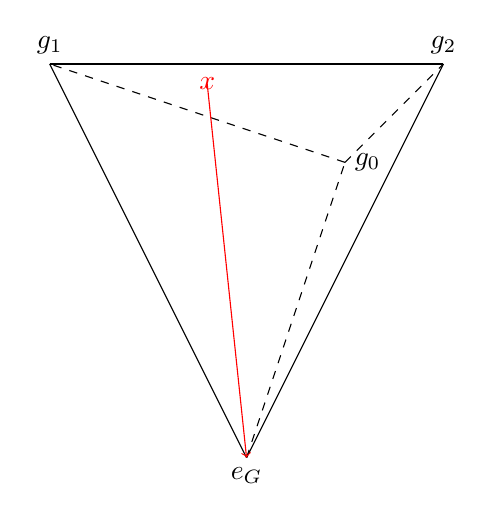
\begin{tikzpicture}[scale=1.25]
  \draw[dashed]
    (0,0) node[below] {$e_{G}$}
    --
    (1,3) node[right] {$g_{0}$};
  \draw
    (0,0)
    --
    (-2,4) node[above] {$g_{1}$};
  \draw
    (0,0)
    --
    (2,4) node[above] {$g_{2}$};
  \draw
    (-2,4)
    --
    (2,4);
  \draw[dashed]
    (1,3)
    --
    (-2,4);
  \draw[dashed]
    (1,3)
    --
    (2,4);
  \draw[->,red]
    (-0.4,3.8) node {$x$}
    --
    (0,0);
\end{tikzpicture}
\]
Note that in the case $e_{G} = g_{0}$ we get a loop in this example. Secondly, the notation  $\mathrm{E}G \slash G$ is not an unfortunate coincidence with that of the orbit space of a group action. For if we topologize $G$ by its power set and $\sim$ is the equivalence relation resulting from the continuous action $\ell_{\mathbf{Top}}$ induced by $\vert \cdot \vert \circ \ell$ then
\begin{align*}
  \mathrm{E}G
  \slash
  G
  &=
  \mathrm{E}G
  \slash
  \sim
\end{align*}
$\ell_{\mathbf{Top}}$ is a \textit{covering space action}\footnote{some say properly discontinuous action} on $\mathrm{E}G$. Since $\mathrm{E}G$ is contractible this means:
\begin{enumerate}
\item[$\bullet$]
the quotient map $\pi_{\ell_{\mathbf{Top}}}$ from $\mathrm{E}G$ to $\mathrm{E}G \slash \sim$ is a \textit{universal}\footnote{this has, in fact, to do with the notion from section \ref{sec:uni}} cover of $\mathrm{E}G \slash \sim$ with discrete fiber $G$ - that is, one whose total space is simply-connected which in turn means the $0$-th and $1$-st homotopy groups are trivial - since $\mathrm{E}G$ as contractible space is clearly simply connected
\item[$\bullet$]
$G$ is isomorphic to the fundamental group
\begin{align*}
  \pi_{1}(\mathrm{E}G \slash G)
  &\cong
  \pi_{1}(\mathrm{B}G)
\end{align*}
\end{enumerate}
This is covering space theory is nicely discussed in \cite{8b5861fc}, for example. The discreteness of the fiber plus the contractibility of the total space of $\pi_{\ell_{\mathbf{Top}}}$ imply that
\begin{align*}
  \pi_{n}(\mathrm{E}G \slash G)
\end{align*}
is trivial for $n > 1$ by a \textit{long exact sequence for Serre fibrations} argument also contained in \cite{8b5861fc}. Since $\mathrm{E}G \slash G$ is path-connected - any two points are connected by a path - the only non-trivial homotopy group of $\mathrm{B}G$ is the first and hence $\mathrm{B}G$ is what is called an \textit{Eilenberg-Mac Lane space for $(G,1)$}. Now what we have done here to understand $\mathrm{B}G$ is the so-called {\glqq}bar construction{\grqq} for a group $G$ by emulating the discussion in \cite{8b5861fc} example 1B.7 which essentially does the same as we do for strict simplicial sets. What is not directly contained there is that $\mathrm{B}G$ is an interesting classifying space\footnote{note the discussion in section \ref{sec:uni} about this terminology}. To this end note that $\pi_{\ell_{\mathbf{Top}}}$ is a locally trivial fiber bundle with fiber (the discrete group) $G$ over the orbit space $\mathrm{E}G \slash G$ resulting from a free continuous action $\ell_{\mathbf{Top}}$ by $G$ on the total space $\mathrm{E}G$ which acts clearly transitively on the fiber since the base space is the quotient space. Thus $\ell_{\mathbf{Top}}$ is a $G$-principal bundle. And this is what $\mathrm{B}G$ can be shown to classify. Namely: homotopy classes of continuous functions from some CW complex $X$ to $\mathrm{B}G$ (which is also a CW complex by theorem \ref{thm:ssetcwcompex}) correspond to isomorphism classes of $G$-principal bundles over $X$. We do not show this here. But it is an easy consequence of a fact proven in \cite{4dc38f27} which in particular implies that $G$-principal bundles with contractible total space are universal elements. The theorem from \cite{4dc38f27} we are talking about more generally applies to arbitrary topological groups and the harder part is in fact to find a universal element for such a topological group. We partly solved this task essentially with categorical means for groups with the discrete topology here. Let us now clearly formulate the statement for general topological groups and refer to proofs:
\\
\begin{thm}
\label{thm:repofbundlefunc}
Assume a group object $G$ in $\mathbf{Top}$ and define the functor
\begin{align*}
  \mathcal{P}_{G}
  \colon
  \left(
    \mathbf{HTop}^{\textrm{CW}}
  \right)^{\mathrm{op}}
  &\rightarrow
  \mathbf{Set}
\end{align*}
by
\begin{enumerate}
\item[$\bullet$]
mapping CW complexes $X$ to the set of isomorphism classes\footnote{the equivalence class w.r.t. the equivalence relation of being an isomorphism} of $G$-principal bundles with base space $X$
\item[$\bullet$]
mapping homotopy classes $[f_{12}] \colon X_{1} \rightarrow X_{2}$ to the isomorphism class of the pullback bundle $f_{12}^{\ast}(p)$ of $[p] \in \mathcal{P}_{G}(X_{2})$ along $f_{12}$
\end{enumerate}
Then $\mathcal{P}_{G}$ is representable.
\end{thm}
\begin{prf}
As pointed out this is proven in \cite{4dc38f27}. But it might also interest you that \cite{6d9ad807} constructs a classifying space for every topological group using simplicial spaces and nerves. 
\\
\phantom{proven}
\hfill
$\square$
\end{prf}
We want to emphasize that $\mathrm{hom}_{\mathbf{HTop}^{\textrm{CW}}}(\cdot,\mathrm{B}G)$ should remind us of cohomology in the light of example \ref{exa:loopradjoint}. And, in fact, $\mathrm{B}G$ is part of a certain $\Omega$-spectrum. But we do not want to elaborate on that further at this point. After all, we call $\mathrm{B}$ the \textbf{classifying space functor} and
\begin{align*}
  \mathrm{B}
  \mathbf{C}
  &\doteq
  \mathrm{B}(\mathbf{C})
\end{align*}
the \textbf{(categorical) classifying space (of $\mathbf{C}$)}. Besides that this generalizes classifying space for $G$-principal bundles with $G$ a discrete space in a canonical way (why should we restrict ourselves to delooping groupoids and not allow arbitrary categories?) we cannot directly be sure that $\mathrm{B}\mathbf{C}$ classifies a sensible mathematical construction in general and thus deserves the terminology. But there seems to be a more or less useful notion which is a certain kind of torsor. So we opted for this terminology here.
\\
To finally convince the reader of the (mathematical) importance of the classifying space functor we want to remark that $\pi_{n} \circ B$ - $\pi_{n}$ is the $n$-th homotopy group functor - applied to a certain kind of category (capturing some properties of exact sequences) is the $n$-the K-group of Quillens algebraic K-theory which is of major importance in algebraic geometry.
\\\\
Lastly, one might wonder why the nerve is called nerve and if you know cohomology you may know that this terminology is also used when it comes to what is traditionally called \v{C}ech cohomology. In fact, our nerve yields the one there more or less directly. According to \cite{wiki-nlab0000} the nerve functor $\mathrm{n}$ is due to Grothendieck who abstracted the so-called \textit{nerve of an open cover} which we will however call \textit{Alexandrov nerve} for reasons of clarity and comprehensibility since from our perspective the \textit{nerve of an open cover} would rather be
\begin{align*}
  \mathrm{n}
  \left(
    \mathbf{Open}_{S}^{\mathrm{cov}_{S}}
  \right)
\end{align*}
But this does not seem to be quite directly what Alexandrov meant.\footnote{though this is claimed in \cite{wiki-pedia0en}:nerve (category theory)} Yet it seems that the \textit{Alexandrov nerve} can in some sense be obtained as nerve in almost this way. Moreover it can be obtained from the \textit{(\v{C}ech) nerve} which is a sort of a nerve in our sense but in a more general setting. You see, things are complicated here and we think literature is quite Kafkaesque on this subject. Especially relating the \v{C}ech nerve to the traditional idea seems hard to find explicitly in literature (as far as we know) and for the sake of simplicity we will not discuss it at this point. But we try to tidy up the rest a bit as far as our understanding allows. So let $S$ be a topological space and
\begin{align*}
  \mathrm{cov}_{S}
  \colon
  K
  &\rightarrow
  \mathrm{ob}_{\mathbf{Open}_{S}}
\end{align*}
be an open cover generator for what follows.
\\
First of all we call
\begin{align*}
  \mathrm{n}
  \left(
    \mathbf{Open}_{S}^{\mathrm{cov}_{S}}
  \right)
\end{align*}
\textbf{nerve (of $\mathrm{cov}_{S}$)} though we will not use this a bit misleading terminology much.
\\
Secondly, we want to introduce the Alexandrov nerve of an open cover which is what is actually called nerve of an open cover. This seems to be historically the first idea which was referred to as nerve of something. The idea is to use $\mathrm{cov}_{S}$ to find a good combinatorial approximation of $S$. More precisely, what Alexandrov seems to have invented is a \textit{(combinatorial) simplicial complex} with vertices ($0$-simplices) just the members of the cover, that is, a vertex for each $k \in K$ or better say $U_{k} \doteq \mathrm{cov}_{S}(k)$. Next take for each non-empty intersection $U_{k_{1}} \cap U_{k_{2}}$ of cover members such that $U_{k_{1}} \neq U_{k_{2}}$ an edge ($1$-simplex) and carry on like that for higher simplices. This is to say for each $n \in \mathbb{N}$ the set of $n$-simplices shall be in bijective correspondence to the set
\begin{align*}
  F_{n}^{\mathrm{cov}_{S}}
  &:=
  \left\lbrace
      U
      \in
      \mathfrak{T}_{S}
    \,
    \vert
    \,
      \exists
      k_{1},
      \ldots
      k_{n+1}
      \in
      K
      \text{ such that }
      U
      =
      U_{k_{1}}
      \cap
      \cdots
      \cap
      U_{k_{n+1}}
      \neq
      \emptyset
      \text{ and }
      U_{k_{1}}
      \neq
      \cdots
      \neq
      U_{k_{n+1}}
  \right\rbrace
\end{align*}
If one knows what a \textit{(combinatorial) simplicial complex} is it is not too hard to see that this defines one. But actually the reader is not expected to know this. Let us geometrically allude to what this means for low dimensional simplices. Namely for vertices, edges and triangles which is sometimes also referred to as $2$-skeleton of the simplicial complex. The dotted area is the simplicial complex corresponding to the space covered by the disks delimited by the circles.
\[
\begin{tikzpicture}[scale=0.75]
  \coordinate (u1) at (0,-1);
  \coordinate (u2) at (-4,0);
  \coordinate (u3) at (-4,3);
  \coordinate (u4) at (-2,6);
  \coordinate (u5) at (1,5);
  \coordinate (u6) at (2,2);
  \coordinate (u7) at (4,0);
  \coordinate (u8) at (7,0);
  \draw[dotted,line width=0.8pt]
    (u1)
    --
    (u2)
    --
    (u3)
    --
    (u4)
    --
    (u5)
    --
    (u6);
  \draw[pattern=dots,dotted,line width=0.8pt]
    (u1)
    --
    (u7)
    --
    (u6)
    --
    (u1)
    --
    cycle;
  \draw[dotted,line width=0.8pt]
    (u7)
    --
    (u8);
  \draw
    (u1)
    circle
    [radius=3];
  \draw
    (u2)
    circle
    [radius=2.5];
  \draw
    (u3)
    circle
    [radius=2];
  \draw
    (u4)
    circle
    [radius=2];
  \draw
    (u5)
    circle
    [radius=2];
  \draw
    (u6)
    circle
    [radius=2];
  \draw
    (u7)
    circle
    [radius=2.5];
  \draw
    (u8)
    circle
    [radius=2];
  \filldraw
    (u1)
    circle
    [radius=2pt];
  \filldraw
    (u2)
    circle
    [radius=2pt];
  \filldraw
    (u3)
    circle
    [radius=2pt];
  \filldraw
    (u4)
    circle
    [radius=2pt];
  \filldraw
    (u5)
    circle
    [radius=2pt];
  \filldraw
    (u6)
    circle
    [radius=2pt];
  \filldraw
    (u7)
    circle
    [radius=2pt];
  \filldraw
    (u8)
    circle
    [radius=2pt];
\end{tikzpicture}
\]
Since the circles and all the overlaps of the circles are contractible the geometric simplicial complex has the same homotopy type as the space covered by the circles. Open covers with this contractibility feature are often called \textit{good covers} and the theorem proving this a (weak) homotopy equivalence is often called \textit{nerve theorem}. So depending on the quality of the open cover (and perhaps the space) the \textit{simplicial complex} is a more or less good combinatorial model of the space's homotopy type. This is nice. But we actually want a simplicial set in lieu of a \textit{simplicial complex} for several reasons:
\begin{enumerate}
\item[$\bullet$]
simplicial sets have some perks we have already discussed
\item[$\bullet$]
if we have a simplicial set it could be the nerve of some category and it will be more convenient to apply category theory
\item[$\bullet$]
some readers are perhaps not familiar with simplicial complexes
\end{enumerate}
To make the simplicial complex defined by the sets $F_{n}^{\mathrm{cov}_{S}}$ into a simplicial set modeling $S$ we could totally order the set of vertices $F_{0}^{\mathrm{cov}_{S}}$ to get a so-called \textit{ordered simplicial complex} which is nothing but a strict simplicial set.\footnote{if you do not understand how this works then \cite{4dd1b85f} should produce relief} Dropping the assumption that intersections can only involve different members of the cover yields precisely the degeneracies which we miss to get a simplicial set. Now, if the cover $\mathrm{cov}_{S}$ is finite - that is, if $K$ is finite - this is no problem. Just take the induced order from $\mathbb{N}$ used to prove that $K$ is finite. But in general we have a problem if we want to avoid the axiom of choice. The axiom of choice allows to well-order any set. The drawback is that we then do not know precisely what the simplicial set looks like. But there is a pretty cool trick to avoid the axiom of choice which will also resolve our terminological struggles a bit. Take the \textit{barycentric subdivision}\footnote{this is explained in \cite{8b5861fc}, for example} of the \textit{simplicial complex} associated to the cover generated by $\mathrm{cov}_{S}$. For our illustration this geometrically means to add vertices in every non-empty intersection illustrated by small (red) circles and edges with one end the barycenter of a triangle and the other end a vertex contained in the same triangle illustrated by thin (red) lines according to the following picture.
\[
\begin{tikzpicture}[scale=0.75]
  \coordinate (u1) at (0,-1);
  \coordinate (u2) at (-4,0);
  \coordinate (u3) at (-4,3);
  \coordinate (u4) at (-2,6);
  \coordinate (u5) at (1,5);
  \coordinate (u6) at (2,2);
  \coordinate (u7) at (4,0);
  \coordinate (u8) at (7,0);
  \draw[dotted,line width=0.8pt]
    (u1)
    --
    coordinate[midway](u12)
    (u2)
    --
    coordinate[midway](u23)
    (u3)
    --
    coordinate[midway](u34)
    (u4)
    --
    coordinate[midway](u45)
    (u5)
    --
    coordinate[midway](u56)
    (u6);
  \draw[color=red]
    (u12)
    circle
    [radius=3pt];
  \draw[color=red]
    (u23)
    circle
    [radius=3pt];
  \draw[color=red]
    (u34)
    circle
    [radius=3pt];
  \draw[color=red]
    (u45)
    circle
    [radius=3pt];
  \draw[color=red]
    (u56)
    circle
    [radius=3pt];
  \draw[pattern=dots,dotted,line width=0.8pt]
    (u1)
    --
    coordinate[midway](u17)
    (u7)
    --
    coordinate[midway](u67)
    (u6)
    --
    coordinate[midway](u16)
    (u1);
  \draw[color=red]
    (barycentric cs:u1=1,u7=1,u6=1)
    circle
    [radius=3pt];
  \draw[color=red]
    (u17)
    circle
    [radius=3pt];
  \draw[color=red]
    (u67)
    circle
    [radius=3pt];
  \draw[color=red]
    (u16)
    circle
    [radius=3pt];
  \draw[thin,color=red]
    (u1)
    --
    (u67)
    (u7)
    --
    (u16)
    (u6)
    --
    (u17);
  \draw[dotted,line width=0.8pt]
    (u7)
    --
    coordinate[midway](u78)
    (u8);
  \draw[color=red]
    (u78)
    circle
    [radius=3pt];
  \draw
    (u1)
    circle
    [radius=3];
  \draw
    (u2)
    circle
    [radius=2.5];
  \draw
    (u3)
    circle
    [radius=2];
  \draw
    (u4)
    circle
    [radius=2];
  \draw
    (u5)
    circle
    [radius=2];
  \draw
    (u6)
    circle
    [radius=2];
  \draw
    (u7)
    circle
    [radius=2.5];
  \draw
    (u8)
    circle
    [radius=2];
  \filldraw
    (u1)
    circle
    [radius=2pt];
  \filldraw
    (u2)
    circle
    [radius=2pt];
  \filldraw
    (u3)
    circle
    [radius=2pt];
  \filldraw
    (u4)
    circle
    [radius=2pt];
  \filldraw
    (u5)
    circle
    [radius=2pt];
  \filldraw
    (u6)
    circle
    [radius=2pt];
  \filldraw
    (u7)
    circle
    [radius=2pt];
  \filldraw
    (u8)
    circle
    [radius=2pt];
\end{tikzpicture}
\]
The point is that the barycentric subdivision of a simplicial complex does not change its homotopy type and that to each intersection of distinct cover members there is a corresponding unique vertex of the barycentric subdivision of the simplicial complex in such a way that for any two vertices connected by an edge precisely one of them correponds to an intersection which can be included in the cover member corresponding to the other vertex. And this inclusion can be used to say which vertex is {\glqq}smaller{\grqq}. We claim the natural convention is that the vertex corresponding to the smaller (as a subset) set is the smaller vertex and indicate this by an arrow $\rightarrow$ which means ordered by inclusion in the following picture.
\[
\begin{tikzpicture}[scale=0.75]
  \coordinate (u1) at (0,-1);
  \coordinate (u2) at (-4,0);
  \coordinate (u3) at (-4,3);
  \coordinate (u4) at (-2,6);
  \coordinate (u5) at (1,5);
  \coordinate (u6) at (2,2);
  \coordinate (u7) at (4,0);
  \coordinate (u8) at (7,0);
  \draw[color=white]
    (u1)
    --
    coordinate[midway](u12)
    (u2)
    --
    coordinate[midway](u23)
    (u3)
    --
    coordinate[midway](u34)
    (u4)
    --
    coordinate[midway](u45)
    (u5)
    --
    coordinate[midway](u56)
    (u6);
  \filldraw[color=white,pattern=dots]
    (u1)
    --
    coordinate[midway](u17)
    (u7)
    --
    coordinate[midway](u67)
    (u6)
    --
    coordinate[midway](u16)
    (u1);
  \draw[color=white]
    (u7)
    --
    coordinate[midway](u78)
    (u8);
  \draw[thick,->]
    (u12)
    --
    (u1);
  \draw[thick,->]
    (u12)
    --
    (u2);
  \draw[thick,->]
    (u23)
    --
    (u2);
  \draw[thick,->]
    (u23)
    --
    (u3);
  \draw[thick,->]
    (u34)
    --
    (u3);
  \draw[thick,->]
    (u34)
    --
    (u4);
  \draw[thick,->]
    (u45)
    --
    (u4);
  \draw[thick,->]
    (u45)
    --
    (u5);
  \draw[thick,->]
    (u56)
    --
    (u5);
  \draw[thick,->]
    (u56)
    --
    (u6);
  \draw[thick,->]
    (u67)
    --
    (u6);
  \draw[thick,->]
    (u67)
    --
    (u7);
  \draw[thick,->]
    (u78)
    --
    (u7);
  \draw[thick,->]
    (u78)
    --
    (u8);
  \draw[thick,->]
    (u16)
    --
    (u1);
  \draw[thick,->]
    (u16)
    --
    (u6);
  \draw[thick,->]
    (u17)
    --
    (u1);
  \draw[thick,->]
    (u17)
    --
    (u7);
  \draw[thick,->]
    (barycentric cs:u1=1,u7=1,u6=1)
    --
    (u1);
  \draw[thick,->]
    (barycentric cs:u1=1,u7=1,u6=1)
    --
    (u6);
  \draw[thick,->]
    (barycentric cs:u1=1,u7=1,u6=1)
    --
    (u7);
  \draw[thick,->]
    (barycentric cs:u1=1,u7=1,u6=1)
    --
    (u67);
  \draw[thick,->]
    (barycentric cs:u1=1,u7=1,u6=1)
    --
    (u16);
  \draw[thick,->]
    (barycentric cs:u1=1,u7=1,u6=1)
    --
    (u17);
  \draw
    (u1)
    circle
    [radius=3];
  \draw
    (u2)
    circle
    [radius=2.5];
  \draw
    (u3)
    circle
    [radius=2];
  \draw
    (u4)
    circle
    [radius=2];
  \draw
    (u5)
    circle
    [radius=2];
  \draw
    (u6)
    circle
    [radius=2];
  \draw
    (u7)
    circle
    [radius=2.5];
  \draw
    (u8)
    circle
    [radius=2];
  \filldraw[color=green]
    (u1)
    circle
    [radius=2pt];
  \filldraw[color=green]
    (u2)
    circle
    [radius=2pt];
  \filldraw[color=green]
    (u3)
    circle
    [radius=2pt];
  \filldraw[color=green]
    (u4)
    circle
    [radius=2pt];
  \filldraw[color=green]
    (u5)
    circle
    [radius=2pt];
  \filldraw[color=green]
    (u6)
    circle
    [radius=2pt];
  \filldraw[color=green]
    (u7)
    circle
    [radius=2pt];
  \filldraw[color=green]
    (u8)
    circle
    [radius=2pt];
  \filldraw[color=green]
    (u12)
    circle
    [radius=2pt];
  \filldraw[color=green]
    (u23)
    circle
    [radius=2pt];
  \filldraw[color=green]
    (u34)
    circle
    [radius=2pt];
  \filldraw[color=green]
    (u45)
    circle
    [radius=2pt];
  \filldraw[color=green]
    (u56)
    circle
    [radius=2pt];
  \filldraw[color=green]
    (u67)
    circle
    [radius=2pt];
  \filldraw[color=green]
    (u78)
    circle
    [radius=2pt];
  \filldraw[color=green]
    (u16)
    circle
    [radius=2pt];
  \filldraw[color=green]
    (u17)
    circle
    [radius=2pt];
  \filldraw[color=green]
    (barycentric cs:u1=1,u7=1,u6=1)
    circle
    [radius=2pt];
\end{tikzpicture}
\]
So the barycentric subdivision yields a strict simplicial set which when realized geometrically exhibits the same homotopy type as the geometric simplicial complex. Again, dropping the assumption that intersections can only involve different members of the cover should yield the wanted simplicial set.
\\
We hope you got the gist from this motivational discussion and hope you are able to comprehend the following definitions. From the open cover generator $\mathrm{cov}_{S}$ we get an open cover of $S$ by
\begin{align*}
  \mathfrak{D}_{\mathrm{cov}_{S}}
  &:=
  \left\lbrace
      U
      \in
      \mathfrak{T}_{S}
    \,
    \vert
    \,
      \exists
      n
      \in
      \mathbb{N}^{\times}
      \left(
        \exists
        k_{1},
        \ldots
        k_{n+1}
        \in
        K
        \text{ such that }
        U
        =
        U_{k_{1}}
        \cap
        \cdots
        \cap
        U_{k_{n+1}}
        \neq
        \emptyset
      \right)
  \right\rbrace
\end{align*}
and hence an open cover generator
\begin{align*}
  \cap_{\mathrm{cov}_{S}}
  &:=
  \mathrm{cov}_{S}
  \left[
    \mathfrak{D}_{\mathrm{cov}_{S}}
  \right]
\end{align*}
Then we call
\begin{align*}
  \mathrm{A}_{\mathrm{cov}_{S}}
  &:=
  \mathrm{n}
  \left(
    \mathbf{Open}_{S}^{\cap_{\mathrm{cov}_{S}}}
  \right)
\end{align*}
\textbf{Alexandrov nerve (of $\mathrm{cov}_{S}$)}. We claim that the geometric realization of the Alexandrov nerve is structurally equal to the simplicial set we discussed in the motivation justifying the terminology. But we do not prove that here. However, we tell you that this claim is essentially made by Segal in \cite{6d9ad807}. Unfortunately, in these notes the claim is not explained and we could not further follow back that claim to its origin. So you are on your own for a proof of this.
\\
We already indicated that covers with every member contractible are good in the sense that they may allow a \textit{nerve theorem}. Intuitively, we think this is clear from our drawings above. So let us formalize the notion of good covers. $\mathrm{cov}_{S}$ is called a \textbf{good cover (of $S$)} if any object
\begin{align*}
  U
  &\in
  \mathrm{ob}_{\mathbf{Open}_{S}^{\cap_{\mathrm{cov}_{S}}}}
\end{align*}
is contractible.
\\
Now if one has a simplicial set it is almost mandatory to apply simplicial (co)homology to examine the homotopy properties of its geometric realization. We presuppose a knowledge about simplicial homology and simplicial cohomology for simplicial sets which is essentially the same as the version for strict simplicial sets presented in \cite{8b5861fc}. Moreover we require the reader to be familiar with intuition about cohomology for what follows. See the introduction to chapter 3 of \cite{8b5861fc} to get a feeling for cocycles and coboundaries in low dimensions. You can also look at the according chapter of \cite{00000011} for a quick introduction. Now, to us only the simplicial cohomology matters. So let us briefly revisit what the simplicial cohomology for the Alexandrov nerve of $\mathrm{cov}_{S}$ is. An element of
\begin{align*}
  \mathrm{A}_{\mathrm{cov}_{S}}
  ([N])
\end{align*}
for $N \in \mathbb{N}$ is called \textbf{$N$-simplex (of $\mathrm{cov}_{S}$)} while we denote the free abelian group with generators the $N$-simplices by $\Delta_{N}[S]$ for $N \in \mathbb{N}$. Then for an $N$-simplex $\sigma$ we call
\begin{align*}
  \partial
  \sigma
  &=
  \Sigma_{i=0}^{N}
  (-1)^{i+1}
  d_{N,i}(\sigma)
\end{align*}
regarded as element of $\Delta_{N-1}[S]$ where $d_{N,i}$ is $i$-th face map of the $N$ simplices in
\begin{align*}
  \mathrm{A}_{\mathrm{cov}_{S}}
\end{align*}
the \textbf{boundary of $\sigma$}. The boundaries of all the $N$-simplices define a homomorphism $\partial_{N}$ on all of $\Delta_{N}[S]$ since it suffices to determine a homomorphism on generators. We call $\partial_{N}$ the \textbf{$N$-boundary operator} Then for some abelian group $A$ the contravariant hom-functor
\begin{align*}
  \partial^{N}
  \doteq
  \partial_{A}^{N}
  :=
  \mathrm{hom}_{\mathbf{Ab}}(\partial_{N+1},A)
  \colon
  \mathrm{mor}_{\mathbf{Ab}}
  \left(
    \Delta_{N}[S],
    A
  \right)
  &\rightarrow
  \mathrm{mor}_{\mathbf{Ab}}
  \left(
    \Delta_{N+1}[S],
    A
  \right)
\end{align*}
is called \textbf{$N$-coboundary operator}. The abelian groups
\begin{align*}
  \mathrm{mor}_{\mathbf{Ab}}
  \left(
    \Delta_{N}[S],
    A
  \right)
\end{align*}
define a cochain complex with cohomology groups
\begin{align*}
  \check{H}_{A}^{N}
  \left(
    \mathrm{A}_{\mathrm{cov}_{S}}
  \right)
  &:=
  \mathrm{ker}
  \left(
    \partial^{N}
  \right)
  \slash
  \mathrm{im}
  \left(
    \partial^{N-1}
  \right)
\end{align*}
for $N \in \mathbb{N}^{\times}$ and
\begin{align*}
  \check{H}_{A}^{0}
  \left(
    \mathrm{A}_{\mathrm{cov}_{S}}
  \right)
  &:=
  \mathrm{ker}
  \left(
    \partial^{0}
  \right)
\end{align*}
where $\mathrm{ker}$ and $\mathrm{im}$ mean \textit{kernel} and \textit{image}, respectively. For $N \in \mathbb{N}$ 
\begin{align*}
  \check{H}_{A}^{N}
  \left(
    \mathrm{A}_{\mathrm{cov}_{S}}
  \right)
\end{align*}
is called \textbf{$N$-th \v{C}ech cohomology group (of $\mathrm{cov}_{S}$ with coefficients in $A$)}. So far, so good. But we actually want a cohomology for $S$ and not for its cover. So what are our options? By the nerve theorem we should get a reasonable cohomology if we take a cover fulfilling the conditions of the nerve theorem. So the \v{C}ech cohomology group for a good cover should in certain cases yield some homotopy properties of $S$. But there is another more indirect approach. In subsection \ref{sec:func} we have said that open covers are ordered as directed set by refinement. So we can take the colimit since $\mathbf{Ab}$ is bicomplete. This is to say we can consider
\begin{align*}
  \check{H}_{A}^{N}
  \left(
    S
  \right)
  &:=
  \varinjlim_{\pmb{\leq}_{\mathrm{Cov}_{S}}}
  \left(
    \check{H}_{A}^{N}
    \left(
      \mathrm{A}_{\mathrm{cov}_{S}}
    \right)
  \right)
\end{align*}
for all $N \in \mathbb{N}$ which we call the \textbf{$N$-th \v{C}ech cohomology group (of $S$ with coefficients in $A$)}. The idea is that the Alexandrov nerve of finer and finer covers eventually is a good approximation of $S$.
\begin{align*}
  \check{H}_{A}^{N}
  \left(
    S
  \right)
\end{align*}
defines an \textit{axiomatic cohomology theory}. It is a well-known fact that for $S$ a CW complex
\begin{align*}
  \check{H}_{A}^{N}
  \left(
    S
  \right)
\end{align*}
is the same as \textit{singular cohomology for $S$ with coefficients in $A$} when compared as axiomatic cohomology theory on this category of nice spaces. Furthermore for $S \in \mathrm{ob}_{\mathbf{Diff}_{\infty}}$ the same is true for \textit{de Rham cohomology for $S$ with coefficients in $\mathbb{R}$}. But note that in the de Rham case we could also use the option of a good cover and its \v{C}ech cohomology since a smooth manifold is locally contractible and hence allows for a good cover. Therefore we want to emphasize that the colimit option is not necessarily better than the good cover option. Indeed, when considering cohomology more generally in the modern $(\infty,1)$-category context the good cover option seems more prevalent. At least when following \cite{a565d200}. There it also becomes clear that \v{C}ech cohomology is more like a method to calculate other cohomologies as we tried to suggest by relating it to singular and de Rham cohomology. Let us give a foretaste of what we mean. Above in theorem \ref{thm:repofbundlefunc} we had that isomorphism classes of $G$-principal bundles over some CW Complex $S$ are classified by morphisms from $S$ into the Eilenberg-Mac Lane space $\mathrm{B}G$. These morphisms in turn can be shown to correspond to the elements of the first singular cohomology for $S$ with coefficients $G$ if $G$ is an abelian group by the machinery alluded to in example \ref{exa:loopradjoint} (when taking base points into account). Hence the first \v{C}ech cohomology can be used to classify the addressed bundles over $S$. Therefore it seems instructive to take a closer look at
\begin{align*}
  \check{H}_{A}^{N}
  \left(
    \mathrm{A}_{\mathrm{cov}_{S}}
  \right)
\end{align*}
Well, an abelian group homomorphism
\begin{align*}
  \phi
  \colon
  \Delta_{1}[S]
  &\rightarrow
  A
\end{align*}
is precisely a $1$-cocycle (that is, an element of the kernel of $\partial^{1}$) if for any\footnote{note that $\sigma$ here is rather for \underline{s}implex than for \underline{s}ection and in the light of example \ref{exa:bundles2} an unfortunate coincidence}
\begin{align*}
  \sigma
  &\in
  \mathrm{A}_{\mathrm{cov}_{S}}
  ([2])
\end{align*}
we have
\begin{align*}
  \phi
  \left(
    d_{2,2}(\sigma)
  \right)
  =
  &\phi
  \left(
    d_{2,3}(\sigma)
  \right)
  \cdot_{A}
  \phi
  \left(
    d_{2,1}(\sigma)
  \right)
\end{align*}
which is sometimes referred to as ($1$-)cocycle condition\footnote{here is where it is worthwhile to know the motivation for cohomology \cite{8b5861fc}}. Let us emphasize that we also had that in our bundles 2 example \ref{exa:bundles2}. The first cohomology class is obtained by identifying $1$-cocycles $\phi$ and $\phi^{\backprime}$ if there is a $0$-cocycle
\begin{align*}
  a
  \colon
  \Delta_{0}[S]
  &\rightarrow
  A
\end{align*}
such that
\begin{align*}
  \phi(\sigma)
  &=
  \phi^{\backprime}(\sigma)
  \cdot_{A}
  \left(
    \partial^{0}
    \left(
      a
    \right)
  \right)
  (\sigma)
\end{align*}
for all
\begin{align*}
  \sigma
  &\in
  \mathrm{A}_{\mathrm{cov}_{S}}
  ([1])
\end{align*}
which can equivalently be expressed as
\begin{align*}
  \phi(\sigma)
  &=
  \phi^{\backprime}(\sigma)
  \cdot_{A}
  a
  \left(
    d_{1,1}(\sigma)
    -
    d_{1,0}(\sigma)
  \right)
\end{align*}
which in turn is the same as
\begin{align*}
  a
  \left(
    d_{1,0}(\sigma)
  \right)
  \cdot_{A}
  \phi(\sigma)
  &=
  \phi^{\backprime}(\sigma)
  \cdot_{A}
  a
  \left(
    d_{1,1}(\sigma)
  \right)
\end{align*}
since $A$ is abelian. We identify this as the formal coboundary condition from example \ref{exa:bundles2}. The idea now is, since we treat the space $S$ by coverings, to take the coefficients only locally to get a finer notion of \v{C}ech cohomology. For a consistent choice of local coefficients it seems reasonable to take a sheaf of coefficients. This is to say an \textit{abelian} group object in $\mathbf{Sh}(S)$. It is not much trouble to make this work to yield a more general version of the \v{C}ech cohomology we presented here. The ordinary case is contained as the special case with the so-called \textit{contant sheaf (on $S$ determined by $A$)} in the more general one. By constant sheaf we just mean the sheafification (see example \ref{exa:sheafetale}) of the presheaf which maps any open subspace of $S$ to $A$ while restriction is just identity. One only has to take care of restrictions along inclusions a bit. How this works in detail can be found on \cite{wiki-pedia0en}: \v{C}ech cohomology. We will only look at the case of the first \v{C}ech cohomology group in the more general non-abelian case. This non-abelian (\v{C}ech) cohomology is important since for $G$-principal bundles $G$ is in general not abelian. What we essentially do to generalize first \v{C}ech cohomology is replacing the topological group $G$ by a group object in $\mathbf{Sh}(S)$ which is then a generalized space. Hence a final example for this section prolonging the generalized spaces example from examples \ref{exa:gs1} and \ref{exa:gs2}.
\\
\begin{exa}[Generalized Spaces III]
\label{exa:gs3}
In the following assume that $G$ is a group object in $\mathbf{Sh}(S)$ w.r.t. some $(\mathrm{m},\mathrm{id},\mathrm{inv})$. This in particular means that we locally have groups
\begin{align*}
  \left(
    G(U),
    \mathrm{m}(U),
    \mathrm{id}(U),
    \mathrm{inv}(U)
  \right)
\end{align*}
for $U \in \mathrm{ob}_{\mathbf{Open}_{S}}$. But for different objects $U_{1},U_{2} \in \mathrm{ob}_{\mathbf{Open}_{S}}$ we do not necessarily have that $G(U_{1})$ equals $G(U_{2})$ we only have a restriction (in the guise of a group homomorphism) from $G(U_{2})$ to $G(U_{1})$ if and only if $U_{1} \subset U_{2}$. Thus the cocycle condition does not quite make sense directly anymore since each term of this condition is potentially in a different group and we should restrict the terms to the largest possible common domain, that is, the intersection of all the domains involved. So let
\begin{align*}
  \sigma
  &\in
  \mathrm{A}_{\mathrm{cov}_{S}}([2])
\end{align*}
Note that $\sigma$ is a functor on $\pmb{\leq}_{[2]}$ and hence use the notation
\begin{align*}
  U_{k}
  &\doteq
  \sigma(k)
  \in
  \mathrm{ob}_{\mathbf{Open}_{S}^{\cap_{\mathrm{cov}_{S}}}}
  \\
  U_{1}
  \cap_{\textrm{f}}
  U_{2}
  &\doteq
  d_{2,3}(\sigma)
  \\
  U_{2}
  \cap_{\textrm{f}}
  U_{3}
  &\doteq
  d_{2,1}(\sigma)
  \\
  U_{1}
  \cap_{\textrm{f}}
  U_{3}
  &\doteq
  d_{2,2}(\sigma)
\end{align*}
for $k = 1,2,3$ as well as
\begin{align*}
  \mathrm{i}_{1}
  &\in
  \mathrm{mor}_{\mathbf{Open}_{S}}
  \left(
    U_{1}
    \cap
    U_{2}
    \cap
    U_{3},
    U_{2}
    \cap
    U_{3}
  \right)
  \\
  \mathrm{i}_{2}
  &\in
  \mathrm{mor}_{\mathbf{Open}_{S}}
  \left(
    U_{1}
    \cap
    U_{2}
    \cap
    U_{3},
    U_{1}
    \cap
    U_{3}
  \right)
  \\
  \mathrm{i}_{3}
  &\in
  \mathrm{mor}_{\mathbf{Open}_{S}}
  \left(
    U_{1}
    \cap
    U_{2}
    \cap
    U_{3},
    U_{1}
    \cap
    U_{2}
  \right)
\end{align*}
Then we call a dependent function
\begin{align*}
  \phi
  &\in
  \prod_{\sigma^{\backprime} \in \mathrm{A}_{\mathrm{cov}_{S}}([1])}
  G(\sigma^{\backprime}(1) \cap \sigma^{\backprime}(2))
\end{align*}
a \textbf{$1$-cocycle (for $\mathrm{cov}_{S}$ with coefficients in $G$)} if
\begin{align*}
  G(\mathrm{i}_{2})
  \left(
    \phi(U_{1} \cap_{\textrm{f}} U_{3})
  \right)
  &=
  \left(
    \mathrm{m}
    \left(
      U_{1}
      \cap
      U_{2}
      \cap
      U_{3}
    \right)
  \right)
  \left(
    G(\mathrm{i}_{3})
    \left(
      \phi(U_{1} \cap_{\textrm{f}} U_{2})
    \right),
    G(\mathrm{i}_{1})
    \left(
      \phi(U_{2} \cap_{\textrm{f}} U_{3})
    \right)
  \right)
\end{align*}
which we abbreviate
\begin{align*}
  \phi(U_{1} \cap_{\textrm{f}} U_{3})
  &=
  \phi(U_{1} \cap_{\textrm{f}} U_{2})
  \phi(U_{2} \cap_{\textrm{f}} U_{3})
\end{align*}
for all
\begin{align*}
  \sigma
  &\in
  \mathrm{A}_{\mathrm{cov}_{S}}([2])
\end{align*}
Moreover we define an equivalence relation $\sim$ on the set of $1$-cocycles by
\begin{align*}
  \phi
  &\sim
  \phi^{\backprime}
\end{align*}
for
\begin{align*}
  \phi,
  \phi^{\backprime}
  &\in
  \prod_{\sigma^{\backprime} \in \mathrm{A}_{\mathrm{cov}_{S}}([1])}
  G(\sigma^{\backprime}(1) \cap \sigma^{\backprime}(2))
\end{align*}
if and only if there is
\begin{align*}
  f
  \in
  \prod_{\sigma^{\backprime} \in \mathrm{A}_{\mathrm{cov}_{S}}([0])}
  G(\sigma^{\backprime}(1))
\end{align*}
such that
\begin{align*}
  f(U_{1})
  \phi(U_{1} \cap_{\textrm{f}} U_{2})
  =
  \phi^{\backprime}(U_{1} \cap_{\textrm{f}} U_{2})
  f(U_{2})
\end{align*}
with a simliar notational convention as for the cocycle condition to handle restriction and multiplication economically. We have to admit that this coboundary condition is a bit arbitrarily abstracted from the constant and abelian case but we feel emboldened for this by the observations in example \ref{exa:bundles2} about the principal bundles. Moreover it seems to later fit to cohomology in the $(\infty,1)$-categorical context vindicating it a bit a posteriori or so. Either way the rest of the example works with this choice. Now what is left to make this first non-abelian \v{C}ech generalization deserving the name is to either look at good covers or let the equivalence classes vary with the directed system of covers. The first option is quite clear. For the latter define the functor
\begin{align*}
  H_{G}^{1}
  \colon
  \pmb{\leq}_{\mathrm{Cov}_{S}}
  &\rightarrow
  \mathbf{Grp}^{\mathrm{op}}
  \\
  \mathrm{cov}_{S}
  &\mapsto
  \left.
    \left(
      \prod_{\sigma^{\backprime} \in \mathrm{A}_{\mathrm{cov}_{S}}([1])}
      G(\sigma^{\backprime}(1) \cap \sigma^{\backprime}(2))
    \right)
  \right\slash
  \sim
  \\
  \left(
    \mathrm{cov}_{S}^{\alpha},
    \mathrm{cov}_{S}
  \right)
  &\mapsto
  \left(
    [\phi]
    \mapsto
    \left[
      \sigma^{\alpha}
      \mapsto
      G(\mathrm{i}_{\sigma^{\alpha},\sigma^{\backprime}})
      (\phi(\sigma^{\backprime}))
    \right]
  \right)
\end{align*}
where
\begin{align*}
  \mathrm{i}_{\sigma^{\alpha},\sigma^{\backprime}}
  &\in
  \mathrm{mor}_{\mathbf{Open}_{S}}
  \left(
    \sigma^{\alpha}(1)
    \cap
    \sigma^{\alpha}(2),
    \sigma^{\backprime}(1)
    \cap
    \sigma^{\backprime}(2)
  \right)
\end{align*}
is from a choice we can make by the refinement property. Now we can apply the colimit functor (since $\mathbf{Grp}$ is a bicomplete category) to get a generalized version of \v{C}ech cohomology. In the one-dimensional case at least. 
\begin{align*}
  \check{H}_{G}^{1}(S)
  &:=
  \varinjlim_{\pmb{\leq}_{\mathrm{Cov}_{S}}}
  \left(
    H_{G}^{1}
  \right)
\end{align*}
is called the \textbf{$1$-st \v{C}ech cohomology group (of $S$ with coefficients in $G$)}. Note that $G$ is a sheaf here as group object in the topos of sheaves $\mathbf{Sh}(S)$. What we should now do is to construct from a cocycle the thing it classifies in an intuitive manner. We are sorry that we are not able to directly do this here. We just do not know how this goes although we tried hard. Therefore we only tell you what it classifies: the $1$-st \v{C}ech cohomology group classifies isormophism classes of right $G$-torsors in $\mathbf{Sh}(S)$. For a proof sketch of this fact you can look at \cite{c82f5e22}. Note that example \ref{exa:gs4} in section \ref{sec:fibration}, the sequel to this example, is a also based on a part of \cite{c82f5e22}. Anyways, the proof sketch there utilizes the equivalence of sheaves and \'{e}tale bundles from example \ref{exa:sheafetale} which we actually wanted to avoid. Yet, we can recommend the proof to gain some insight since the perspective as bundle is not the wrong in the end. What is interesting here is that the traditional $1$-st \v{C}ech cohomology group classifies loosly speaking torsors in the slice category $\mathbf{Top} \slash S$ with a certain local triviality property while the generalized version of $1$-st \v{C}ech cohomology group classifies torsors in $\mathbf{Sh}(S)$. At first glance it seems as we somehow have forgotton the local triviality by generalizing. But note that sheaves themselves capture local triviality in some sense. That this is sensible can be seen in the case of discrete topological groups $G$ for which the $G$-principal bundles correspond to $\bar{G}$-torsors where $\bar{G}$ is the constant sheaf determined by $G$. A discussion can be found in \cite{c55c71e8} in the classifying topoi chapter.
\iffalse
Now let
\begin{align*}
  \phi
  &\in
  \prod_{\sigma^{\backprime} \in \mathrm{A}_{\mathrm{cov}_{S}}([1])}
  G(\sigma^{\backprime}(1) \cap \sigma^{\backprime}(2))
\end{align*}
be a $1$-cocycle for $\mathrm{cov}_{S}$ with coefficients in $G$. Then $\phi$ induces a bijection from $G(U_{k})$ to $G(U_{k})$ for all $k \in K$ by right multiplication with $\phi(\sigma_{k})$ where $\sigma_{k} \in \mathrm{A}_{\mathrm{cov}_{S}}([1])$ denotes the degenerate $1$-simplex for $U_{k}$, that is,
\begin{align*}
  U_{k}
  &=
  \sigma_{k}(1)
  =
  \sigma_{k}(2)
\end{align*}
This is to say the function
\begin{align*}
  r_{\phi(\sigma_{k})}
  \colon
  G(U_{k})
  &\rightarrow
  G(U_{k})
  \\
  g
  &\mapsto
  g
  \cdot_{G(U_{k})}
  \phi(\sigma_{k})
\end{align*}
is a bijection.\footnote{this can be made into a group automorphism by considering $\phi(\sigma_{k})$ as identity of the codomain while the domain still has the old identity} Now let $V \subset U_{k}$ and $\mathrm{i}_{V}$ the inclusion into $U_{k}$. Then we have a group homomorphism $G(\mathrm{i}_{V})$ from $G(U_{k})$ to $G(V)$ since $G$ is a sheaf in groups. Moreover we get a bijection
\begin{align*}
  r_{G(\mathrm{i}_{V})(\phi(\sigma_{k}))}
  \colon
  G(V)
  &\rightarrow
  G(V)
  \\
  g
  &\mapsto
  g
  \cdot_{G(V)}
  G(\mathrm{i}_{V})
  \left(
    \phi(\sigma_{k})
  \right)
\end{align*}
such that
\begin{align*}
  r_{G(\mathrm{i}_{V})(\phi(\sigma_{k}))}
  \left(
    G(\mathrm{i}_{V})(g)
  \right)
  &=
  G(\mathrm{i}_{V})(g)
  \cdot_{G(V)}
  G(\mathrm{i}_{V})
  \left(
    \phi(\sigma_{k})
  \right)
  \\
  &=
  G(\mathrm{i}_{V})
  \left(
    g
    \cdot_{G(U_{k})}
    \phi(\sigma_{k})
  \right)
  \\
  &=
  G(\mathrm{i}_{V})
  \left(
    r_{\phi(\sigma_{k})}(g)
  \right)
\end{align*}
for all $g \in G(U_{k})$ since $G(\mathrm{i}_{V})$ is a group homomorphism. Thus one can show that $r_{\phi(\sigma_{k})}$ defines a sheaf isomorphism $r_{\phi}$ (natural isomorphism) from $G$ restricted to $\mathbf{Open}_{U_{K}}$ to itself by setting
\begin{align*}
  r_{\phi}(V)
  &:=
  r_{G(\mathrm{i}_{V})(\phi(\sigma_{k}))}
\end{align*}
But this corresponds to a sheaf isomorphism $\mathsf{r}_{\phi}$ from $G$ to $G$ such that
\begin{align*}
  \mathsf{r}_{\phi}(U_{k})
  &=
  r_{\phi}(U_{k})
\end{align*}
One can see this in a quite elementary way: any $U \in \mathrm{ob}_{\mathbf{Open}_{S}}$ is covered by all the $U_{k} \cap U$ and then $\mathsf{r}_{\phi}$ is obtained from the universality of the equalizers from the descent condition symbolically illustrated by
\[
\begin{tikzcd}[sep=huge]
  G(U)
  \arrow{r}{\mathrm{eq}}
  \arrow[swap]{d}{\mathsf{r}_{\phi}(U)}
  &
  \prod_{k \in K}
  G(U_{k} \cap U)
  \arrow{d}{\prod_{k \in K}r_{\phi}(U_{k} \cap U)}
  \\
  G(U)
  \arrow{r}{\mathrm{eq}}
  &
  \prod_{k \in K}
  G(U_{k} \cap U)
\end{tikzcd}
\]
So a cocycle $\phi$ yields an isomorphism of sheaves $\mathsf{r}_{\phi}$ from $G$ to $G$ and hence actions
\begin{align*}
  \mathsf{a}_{\phi}(U)
  \colon
  G(U)
  \times
  G(U)
  &\rightarrow
  G(U)
  \\
  (g_{0},g)
  &\mapsto
  \mathsf{r}_{\phi}(U)(g)
  \cdot
  g_{0}
\end{align*}
\fi
\end{exa}
\begin{prf}
For what you do not understand we can only help you by the sources given in the example.
\\
\phantom{proven}
\hfill
$\square$
\end{prf}
